\documentclass[12pt]{article}
\usepackage[a4paper, portrait, margin=1cm, bottom=2cm]{geometry}
\usepackage{fontspec}
\usepackage[fleqn]{amsmath}
\usepackage{amssymb}
\usepackage{graphicx}
\usepackage{indentfirst}
\usepackage{inputenc}[utf8]
\usepackage{polyglossia}
\usepackage[dvipsnames]{xcolor}
\usepackage{svg}
\usepackage{booktabs}
\usepackage{blkarray}
\usepackage[linguistics]{forest}
\usepackage{tikz}
\usetikzlibrary{datavisualization}
\usetikzlibrary{datavisualization.formats.functions}
\usepackage{pgfplots}

\let\gcd\relax
\DeclareMathOperator{\gcd}{НОД}
\DeclareMathOperator{\cd}{ОД}
\DeclareMathOperator{\lcm}{НОК}
\DeclareMathOperator{\cm}{ОК}

\setmainfont[Ligatures=TeX]{Times New Roman}
\setdefaultlanguage{russian}
\setotherlanguages{english}
\graphicspath{graphics}

\begin{document}
\section{Наибольший общий делитель, наименьшее общее кратное и их свойства}
\textbf{Определение.}\par
\begin{tabular}{ccc}
    $a_1,...,a_n \in \mathbb{Z} \, \, \backslash \{0\} \vspace{2 ex}$                                                                                                  \\
    $\{ d|\forall i \ \hspace{2 mm} a_i \ \vdots\ d\} \hspace{2 cm}$ & $d$ - общий делитель$(a_1,...,a_n) \vspace{2 ex}$ & $\gcd(a_1,...a_n) = max \, d \vspace{2 ex}$ \\
    $\{ s|\forall i \ \hspace{2 mm} s \ \vdots\ a_i\} \hspace{2 cm}$ & $s$ - общее кратное$(a_1,...,a_n)$                & НОК$(a_1,...a_n) = min \, s $               \\
\end{tabular}\par

\subsection{Свойства НОД и НОК}
\textbf{Утверждение 1}\par
$\left.\begin{array}{l}
        a_1,...,a_n \in \mathbb{N} \\
        m = \lcm(a_1,...,a_n)      \\
        c  = \cm(a_1,...,a_n)
    \end{array}\right| \Rightarrow c\ \vdots\ m$

\textit{Доказательство:}\par
$\sqsupset c$ не $\ \vdots\ $ на $m$ (от противного)\par
$c = qm+r \hspace{2 cm} 0 < r < m$\par
$\forall i \hspace{1 cm} c \ \vdots\  a_i \hspace{1 cm} m \ \vdots\  a_i$\par
$c-qm \ \vdots\  a_i$\par
$r \ \vdots\  a_i \hspace{1 cm} r$ - ОК$(a_1,...,a_n) \newline$\par

\textbf{Утверждение 2}\par
$a_1,...,a_n \in \mathbb{N}$\par
$d_1,...,d_k$ - все натуральные ОД $(a_1,...,a_n)$\par
НОД$(a_1,...,a_n)=\,$НОК$(d_1,...,d_k) \newline$\par
\textit{Доказательство:}\par
$d_k =\,$ НОД $(a_1,...,a_n)$\par
$a_i \ \vdots\  d_j$\par
$a_i \ \vdots\  \,$ НОК $(d_1,...,d_k)$\par
$d_k \geq \,$ НОК $(d_1,...,d_k)$\par
НОК$(d_1,...,d_k)\ \vdots\  d_k$\par
НОК$(d_1,...,d_k) \geq d_k \newline$\par
Следствие 2-1:\par
\begin{tabular}{ccc}
    $a_1 \ \vdots\  d$                                     \\
    ... & $\Rightarrow$ & НОД $(a_1,...,a_n) \ \vdots\  d$ \\
    $a_n \ \vdots\  d$                                     \\
\end{tabular}\par
\textit{Доказательство следствия:}\par
\begin{tabular}{ccc}
    $\lcm(d_1,...,d_k) \ \vdots\  d_i$ \\
    ||                                 \\
    $\gcd(a_1,...,a_n)$                \\
\end{tabular}\par

\textbf{Утверждение 3.}\par
\begin{enumerate}
    \item $a \ \vdots\  d , \, b \ \vdots\  d \Rightarrow$ НОД $(a,b) \ \vdots\  d$
    \item $s \ \vdots\  a , \, s \ \vdots\  b \Rightarrow s \ \vdots\ $ НОК $(a,b)$
    \item НОД $(a,b)$, НОК $(a,b) = ab$
    \item $bc \ \vdots\  a \hspace{4 mm}$ НОД $(a,b)=d \Rightarrow c \ \vdots\  \frac{a}{d}$
    \item $bc \ \vdots\  a \hspace{4 mm}$ НОД $(a,b)=1 \Rightarrow c \ \vdots\  a$
    \item НОД $(ma, mb) = m$ НОД $(a,b)$
    \item $a \ \vdots\  d, \, b \ \vdots\  d \Rightarrow$ НОД $(\frac{a}{d}, \frac{b}{d}) = \frac{\gcd(a,b)}{d}$
    \item НОД $(a,b) = d \Rightarrow$ НОД $(\frac{a}{d}, \frac{b}{d})=1$
    \item НОД $(a,b)=b \Leftarrow a \ \vdots\  b \hspace{4 mm} a,b \in \mathbb{N}$
    \item НОД $(a+kb,b) =$ НОД $(a,b) \hspace{4 mm} \forall k \in \mathbb{Z}$
\end{enumerate}\par
\textit{Доказательства:}\par
\begin{enumerate}
    \item - следствие 2-1
    \item - утверждение 1
    \item
          \begin{tabular}{c|ccc}
              $ab \ \vdots\  a$                                                                                                                           \\
                                & $\Rightarrow$ & $ab \ \vdots\ \lcm(a,b)$                           & $d = \frac{ab}{\lcm(a,b)}$                         \\
              $ab \ \vdots\  b$ &               & $\frac{a}{d} = \frac{\lcm(a,b)}{b} \in \mathbb{Z}$ & $\frac{b}{d} = \frac{\lcm(a,b)}{a} \in \mathbb{Z}$ \\
          \end{tabular}\par
          $\sqsupset d`$ — $\cd(a,b)$\par
          $a \ \vdots\  d`$\par
          $b \ \vdots\  d`$\par
          $\frac{ab}{d`} = \frac{a}{d`}b \ \vdots\  b \hspace{1 cm} \frac{ab}{d`} = \frac{b}{d`}a \ \vdots\  a$\par
          $\frac{ab}{d`}=k \lcm(a,b) = k \frac{ab}{d}\ | \Rightarrow \ d = kd` \ \vdots\  d`$\par
          $|d| \geqslant |d`|$\par
          $d = \gcd(a,b)$\par
    \item $bc \ \vdots\  a \hspace{1 cm} \gcd(a,b) = d \hspace{1 cm} \lcm(a,b) = \frac{ab}{d}$\par
          \begin{tabular}{c|cc}
              $bc \ \vdots\  a$ &               & $bc \ \vdots\  \lcm(a,b)$    \\
                                & $\Rightarrow$                                \\
              $bc \ \vdots\  b$ &               & $bc \ \vdots\  \frac{ab}{d}$ \\
                                &               & $c \ \vdots\  \frac{a}{d}$   \\
          \end{tabular}\par

    \item без доказательтсва\par
    \item $a \ \vdots\ \gcd(a,b)$\par
          $ma \ \vdots\ m \gcd(a,b)$\par
          $mb \ \vdots\ m \gcd(a,b)$\par
          НОД $(ma, mb) \ \vdots\  m\gcd(a,b)$\par
          $d$ — ОД $(ma,mb)$\par
          $\frac{mab}{d} = \frac{ma}{d}b = \frac{mb}{d}a$\par
          $\frac{mab}{d}$ — ОК $(a,b)$\par
          $\frac{mab}{d} \ \vdots\ $ НОК $(a,b) = \frac{ab}{\gcd(a,b)}$\par
          $mab\ \gcd(a,b) \ \vdots\  abd$\par
          $m\ \gcd(a,b) \ \vdots\  d$\par
          $m\ \gcd(a,b) =\ \gcd(ma,mb)$\par
    \item $d\ \gcd(\frac{a}{d}, \frac{b}{d}) = \gcd(a,b)$ через 6\par
    \item $\gcd(\frac{a}{d}, \frac{b}{d}) = \frac{\gcd(a,b)}{d} = \frac{d}{d} = 1$\par
    \item $a \ \vdots\  b$\par
          $b \ \vdots\  b$\par
          $b$ - ОД $(a,b)$\par
          $d$ - ОД $(a,b) \hspace{1 cm} d > b$\par
          $b \ \vdots\  d \hspace{2.5 cm} b \geqslant d \ (\text{противоречие})$\par
    \item $d = \gcd(a,b)$\par
          $b \ \vdots\  d$\par
          $a \ \vdots\  d \hspace{2 cm} a + kb \ \vdots\  d$\par
          $d$ — $\cd(a+kb, b)$\par
          $d`$ — $\cd(a+kb,b)$\par
          $a+kb \ \vdots\  d`$\par
          $b \ \vdots\  d`$\par
          $a +kb-kb \ \vdots\  d`$\par
          $a \ \vdots\  d`\ \Rightarrow\ d`$ — $\cd(a,b)$\par
          $d \geqslant d`$\par
\end{enumerate}\par

\textbf{Утверждение 4.}\par
$\gcd(a, \gcd(b,c)) = \gcd (a,b,c)$\par
\textit{Доказательство:}\par
$\gcd(b,c) = f$\par
$\gcd(a,f) = g$\par
$a\ \vdots\ g$\par
$b\ \vdots\ f\ \vdots\ g$\par
$c\ \vdots\ f\ \vdots\ g$\par
$\sqsupset d$ — $\cd(a, b, c)$\par
$\left.\begin{array}{l}
        b\ \vdots\ d \\
        c\ \vdots\ d \\
    \end{array}\right| \Rightarrow \gcd(b, c) = f \ \vdots\ d$

$\left.\begin{array}{l}
        a \ \vdots\ d \\
        f \ \vdots\ d \\
    \end{array}\right| \Rightarrow \gcd(a, f) = g \ \vdots\ d \ \Rightarrow\ g = \gcd(a, b, c)$

\textbf{Утверждение 5.} $\lcm(a,\lcm(b,c)) = \lcm(a,b,c)$\par
\textit{Доказательство аналогично доказательству утверждения 4}\par
\subsection{Алгоритм нахождения НОД}\par
\subsubsection{Способ 1}
Поиск всех возможных делителей двух чисел и в выбор наибольшего из них. Пример на числах 12 и 9.\par
$12 : 1 = 12$\par
$12 : 2 = 6$\par
$12 : 3 = 4$\par
$12 : 4 = 3$\par
$12 : 5 = 2 \,$\textit{(2 остаток)}\par
$12 : 6 = 2$\par
$12 : 7 = 1 \,$\textit{(5 остаток)}\par
$12 : 8 = 1 \,$\textit{(4 остаток)}\par
$12 : 9 = 1 \,$\textit{(3 остаток)}\par
$12 : 10 = 1 \,$\textit{(2 остаток)}\par
$12 : 11 = 1 \,$\textit{(1 остаток)}\par
$12 : 12 = 1$\par
Теперь для числа 9 сделаем то же самое.\par
$9 : 1 = 9$\par
$9 : 2 = 4$\textit{(1 остаток)}\par
$9 : 3 = 3$\par
$9 : 4 = 2$\textit{(1 остаток)}\par
$9 : 5 = 1$\textit{(4 остаток)}\par
$9 : 6 = 1$\textit{(3 остаток)}\par
$9 : 7 = 1$\textit{(2 остаток)}\par
$9 : 8 = 1$\textit{(1 остаток)}\par
$9 : 9 = 1$\par
Выпишем делите обоих чисел (те, что без остатка).\par
Делители числа 12 - (1 2 3 4 6 12)\par
Делители числа 9 - (1 3 9)\par
Согласно определению, НОДом чисел 12 и 9, является число, на которое 12 и 9 делятся без остатка.\par
НОДом чисел 12 и 9 является число 3.\par
\subsubsection{Способ 2}
Суть данного способа заключается в том, чтобы разложить оба числа на простые множители и перемножить общие из них. Пример на числах 24 и 18.\par
Разложим оба числа на множители.\par
\begin{tabular}{c|c@{\hskip 1cm}c|c}
    \text{Делимое} & \text{Делитель} & \text{Делимое} & \text{Делитель} \\
    24             & 2               & 18             & 2               \\
    12             & 2               & 9              & 3               \\
    6              & 2               & 3              & 3               \\
    3              & 3               & 1                                \\
    1
\end{tabular}\par
Теперь перемножим их общие множители. Смотрим на разложение числа 24. Первый его множитель это 2. Ищем такой же множитель в разложении числа 18 и видим, что он там тоже есть.\par
Снова смотрим на разложение числа 24. Второй его множитель тоже 2. Ищем такой же множитель в разложении числа 18 и видим, что его там второй раз уже нет.\par
Следующая двойка в разложении числа 24 также отсутствует в разложении числа 18.\par
Переходим к последнему множителю в разложении числа 24. Это множитель 3. Ищем такой же множитель в разложении числа 18 и видим, что там он тоже есть.\par
Итак, общими множителями чисел 24 и 18 являются множители 2 и 3. Чтобы получить НОД, эти множители необходимо перемножить: $2 \times 3 = 6$\par
Значит $\gcd(24, 18) = 6$\par
\subsubsection{Способ 3}
Суть данного способа заключается в том, что числа подлежащие поиску наибольшего общего делителя раскладывают на простые множители. Затем из разложения первого числа вычеркивают множители, которые не входят в разложение второго числа. Оставшиеся числа в первом разложении перемножают и получают НОД. Рассмотрим на примере чисел 28 и 16.\par
В первую очередь, раскладываем числа 28 и 16 на простые множители:\par
\begin{tabular}{c|c@{\hskip 1cm}c|c}
    \text{Делимое} & \text{Делитель} & \text{Делимое} & \text{Делитель} \\
    28             & 2               & 16             & 2               \\
    14             & 2               & 8              & 2               \\
    7              & 7               & 4              & 2               \\
    1              &                 & 2              & 2               \\
                   &                 & 1
\end{tabular}\par
Получили два разложения: $2 \times 2 \times 7$ и $2 \times 2 \times 2 \times 2$\par
Теперь из разложения первого числа вычеркнем множители, которые не входят в разложение второго числа. В разложение второго числа не входит семёрка. Её и вычеркнем из первого разложения.\par
Теперь перемножаем оставшиеся множители и получаем НОД: $2 \times 2 = 4$\par
Число 4 является наибольшим общим делителем чисел 28 и 16. Оба этих числа делятся на 4 без остатка:\par
$28 : 4 = 7$\par
$16 : 4 = 4$\par
$\gcd(28,16)=4$\par

\subsection{Алгоритм нахождения НОК}
\subsubsection{Способ 1}
Можно выписать первые кратные двух чисел, а затем выбрать среди этих кратных такое число, которое будет общим для обоих чисел и маленьким. Рассмотрим на примере числа 9 и 12.\par
В первую очередь, найдем первые кратные для числа 9. Чтобы найти кратные для 9, нужно эту девятку поочерёдно умножить на числа от 1 до 9. Получаемые ответы будут кратными для числа 9.\par
$9 \times 1 = 9$\par
$9 \times 2 = 18$\par
$9 \times 3 = 27$\par
$9 \times 4 = 36$\par
$9 \times 5 = 45$\par
$9 \times 6 = 54$\par
$9 \times 7 = 63$\par
$9 \times 8 = 72$\par
$9 \times 9 = 81$\par
Теперь находим кратные для числа 12. Для этого поочерёдно умножим число 12 на все числа 1 до 12:\par
$12 \times 1 = 12$\par
$12 \times 2 = 24$\par
$12 \times 3 = 36$\par
$12 \times 4 = 48$\par
$12 \times 5 = 60$\par
$12 \times 6 = 72$\par
$12 \times 7 = 84$\par
$12 \times 8 = 96$\par
$12 \times 9 = 108$\par
$12 \times 10 = 120$\par
$12 \times 11 = 132$\par
$12 \times 12 = 144$\par
Теперь выпишем кратные обоих чисел:\par
9: 9 18 27 36 45 54 63 72 81\par
12: 12 24 36 48 60 72 84 96 108 120 132 144\par
Найдём общие кратные обоих чисел.\par
Общими кратными для чисел 9 и 12 являются кратные 36 и 72. Наименьшим же из них является 36.\par
Значит наименьшее общее кратное для чисел 9 и 12 это число 36. Данное число делится на 9 и 12 без остатка:\par
$36 : 9 = 4$\par
$36 : 12 = 3$\par
НОК(9 и 12) = 36\par

\subsubsection{Способ 2}
Второй способ заключается в том, что числа для которых ищется наименьшее общее кратное раскладываются на простые множители. Затем выписываются множители, входящие в первое разложение, и добавляют недостающие множители из второго разложения. Полученные множители перемножают и получают НОК.\par
Применим данный способ для предыдущей задачи. Найдём НОК для чисел 9 и 12.\par
Разложим на множители число 9 и 12:\par
\begin{tabular}{c|c@{\hskip 1cm}c|c}
    \text{Делимое} & \text{Делитель} & \text{Делимое} & \text{Делитель} \\
    9              & 3               & 12             & 2               \\
    3              & 3               & 6              & 2               \\
    1              &                 & 3              & 3               \\
                   &                 & 1
\end{tabular}\par
Выпишем первое  разложение и допишем множители из второго разложения, которых нет в первом разложении. В первом разложении нет двух двоек. Допишем и перемножим: $3 \times 3 \times 2 \times 2 = 36$\par
Получили ответ 36. Значит наименьшее общее кратное чисел 9 и 12 это число 36. Данное число делится на 9 и 12 без остатка:\par
$36 : 9 = 4$\par
$36 : 12 = 3$\par
НОК (9 и 12) = 36\par
Говоря простым языком, всё сводится к тому, чтобы организовать новое разложение куда входят оба разложения сразу. Разложением первого числа 9 являлись множители 3 и 3, а разложением второго числа 12 являлись множители 2, 2 и 3.\par
Наша задача состояла в том, чтобы организовать новое разложение куда входило бы разложение числа 9 и разложение числа 12 одновременно. Для этого мы выписали разложение первого числа и дописали туда множители из второго разложения, которых не было в первом разложении. В результате получили новое разложение 3 × 3 × 2 × 2. Нетрудно увидеть воочию, что в него одновременно входят разложение числа 9 и разложение числа 12.\par

\subsubsection{Способ 3}
Он работает при условии, что его ищут для двух чисел и при условии, что уже найден наибольший общий делитель этих чисел.\par
Данный способ разумнее использовать, когда одновременно нужно найти НОД и НОК двух чисел.\par
К примеру, пусть требуется найти НОД и НОК чисел 24 и 12. Сначала найдем НОД этих чисел:\par
\begin{tabular}{c|c@{\hskip 1cm}c|c}
    \text{Делимое} & \text{Делитель} & \text{Делимое} & \text{Делитель} \\
    24             & 2               & 12             & 2               \\
    12             & 2               & 6              & 2               \\
    6              & 2               & 3              & 3               \\
    3              & 3               & 1              &                 \\
    1              &                 &
\end{tabular}\par
Теперь для нахождения наименьшего общего кратного чисел 24 и 12, нужно перемножить эти два числа и полученный результат разделить на их наибольший общий делитель.\par
Итак, перемножим числа 24 и 12. (288)\par
Разделим полученное число 288 на НОД чисел 24 и 12. (288 : 12 = 24)\par
Получили ответ 24. Значит наименьшее общее кратное чисел 24 и 12 равно 24\par
НОК(24 и 12) = 24.\par

\setcounter{section}{1}
\section{Алгоритм Евклида. Линейное представление НОД(?)}

\subsection{Алгоритм Евклида}
\noindent $a, b \in \mathbb{N}$ \\
НОД$(a, b)$ - ? \\
while $b \ne 0$\\
\indent$(a, b) = (b, a \% b)$\\
return a\\
НОД$(a, b) = $ НОД$(a + kb, b)$\\
$k = -[\frac{a}{b}]$\\
НОД$(a, b) = $ НОД$(a -[\frac{a}{b}]b, b) =$ НОД$(a \% b, b)$\\
$a $ \vdots $ $ $b: $ $ $ НОД$(a, b) = b$
% , где $\vec{r_0} \in$ плоскости $\vec{n}$ - {\bf вектор нормы}.

\subsection{Бинарный алгоритм Евклида}
\noindent $a, b \in \mathbb{N}$\\
$i = 0; j = 0;$\\
while $(!(a \& 1))\{$
\par $a \gg = 1;$
\par $i++;$\\ $\}$\\
while $(!(b \& 1))\{$
\par $b \gg = 1;$
\par $j++;$\\ $\}$\\
if$(a > b) \{ t = a; a = b; b = t;\}$\\
while$(a != 0)\{$\\
\indent $b -= a;$\\
\indent while $(!(b \& 1))$ $b \gg = 1;$\\
\indent if $(a > b)\{$\\
\indent\indent t = a;\\
\indent\indent a = b;\\
\indent\indent b = t;\\
\indent $\}$\\
$\}$\\
return $b \ll$ std::min$(i, j);$



\subsection{Расширенный алгоритм Евклида}
\noindent $a, b \in \mathbb{N}$\\
while $b \ne 0$\\
\indent $q = a / b$\\
\indent $(a, b) = (b, a - qb)$\\
\indent $(x, y) = (y, x - qy)$\\
\indent $a - $ НОД\\
\indent $a, b$\\
\indent $(x, y, u, v) = (1, 0, 0, 1)$\\
while $b \ne 0$\\
\indent $q = a / b$\\
\indent $(a, b) = (b, a - qb)$\\
\indent $(x, y, u, v) = (u, v, x - qu, y - qv)$\\
return $(a, x, y)$

\section{Континуанта}
\subsection{Определение}
Введенные понятия цепной дроби и подходящих дробей оказываются
очень полезными для анализа работы алгоритма Евклида. Дадим необходимые обозначения. Рассмотрим трехдиагональный определитель:\par
$\begin{vmatrix}
        q_0    & 1      & 0      & 0      & ...    & 0       & 0       \\
        -1     & q_1    & 1      & 0      & ...    & 0       & 0       \\
        0      & -1     & q_2    & 1      & ...    & 0       & 0       \\
        \vdots & \vdots & \vdots & \vdots & \ddots & \vdots  & \vdots  \\
        0      & 0      & 0      & 0      & ...    & q_{n-2} & 1       \\
        0      & 0      & 0      & 0      & ...    & -1      & q_{n-1}
    \end{vmatrix}$
= $K_n(q_0, q_1, ..., q_{n-1})$

Определитель называют континуантой $n$-го порядка или индекса.


Континуанта индекса $n$ есть многочлен $K_n$($x_1$, ..., $x_n$)\par
Разложим континуанту n-го порядка по последнему столбцу:\par
$K_n$($x_1$, ..., $x_n$) = $x_n K_{n-1}$($x_1$, ..., $x_{n-1}$) + $K_{n-2}$($x_1$, ..., $x_{n-2}$)\par
Отсюда можно задать континуанту рекуррентным соотношением:\par
$K_{-1} = 0$,   $K_0 = 1$, $K_n = x_nK_{n - 1} + K_{n - 2}$ \par
Cоотношение очень напоминает рекуррентные соотношения для числителей и знаменателей подходящих дробей. Это не случайно и две следующие леммы подтверждают предположение о связи континуант и цепных дробей.
\subsection{Лемма 1}
\textbf{Континуанта $K_n(q_0, q_1, . . . , q_{n−1})$ равна сумме всевозможных произведений элементов $q_0, q_1, . . . , q_{n−1}$, одно из которых содержит
    все эти элементы, а другие получаются из него выбрасыванием одной или
    нескольких пар сомножителей с соседними номерами (если выброшены все
    сомножители, то считаем, что осталась 1).}\par
Доказательство. Индукция по $n$. База индукции:\par
$K_1(q_0) = q_0, K_2(q_0, q_1) = \begin{vmatrix}
        q_0 & 1   \\
        -1  & q_1
    \end{vmatrix}= q_0q_1 + 1$\par
и утверждение леммы справедливо для континуант первого и второго порядков.
Шаг индукции. Пусть утверждение леммы справедливо для континуант ($n$−2)-го и ($n$−1)-го порядков. Применив разложение , получим
требуемое. \par

Пример\par
$K_6(q_0, q_1, q_2, q_3, q_4, q_5) = q_0 q_1 q_2 q_3 q_4 q_5 + q_2 q_3 q_4 q_5 + q_0 q_3 q_4 q_5 + q_0 q_1 q_4 q_5 + q_0 q_1 q_2 q_5 + q_0 q_1 q_2 q_3 + q_4 q_5 + q_2 q_5 + q_0 q_5 + q_2 q_3 + q_0 q_3 + q_0 q_1 + 1$\par
Явная связь континуант и цепных дробей впервые была установлена
Эйлером.
\subsection{Лемма Эйлера}
Справедливо тождество\par
$[q_0;q_1,...,q_{n-1}] = \frac{K_n(q_0, q_1, . . . , q_{n−1})}{K_{n-1}(q_1, q_2, . . . , q_{n−1})}$\par

Доказательство. Индукция по n. База индукции:\par
$[q_0;q_1] = q_0 + \frac{1}{q_1} = \frac{q_0q_1 + 1}{q_1} = \frac{K_2(q_0,q_1)}{K_1(q_1)}$\par
Шаг индукции. Пусть тождество верно для дробей с $n$−1 звеном включительно. Представим $n$-звенную дробь $(q_0, q_1, . . . , q_{n−1})$ дробью с $n$−1 звеном, где последнее звено имеет вид $q_{n−2} + \frac{1}{q_{n-1}}$. Применив к этой дроби индукционное предположение, с учетом разложения , имеем\par
$[q_0; q_1, . . . , q_{n−1}] = [q_0, q_1, . . . , q_{n−2} + \frac{1}{q_{n-1}}] = \frac{K_{n-1}(q_0, q_1, . . . , (q_{n-2}+\frac{1}{q_{n-1})})}{K_{n-2}(q_1, q_2, . . . , (q_{n-2}+\frac{1}{q_{n-1})})} = \frac{(\frac{1}{q_{n-1}}) K_{n-2}(q_0,q_1,...,q_{n-3})+K_{n-3}(q_0,q_1,...,q_{n-4})}{(\frac{1}{q_{n-1}}) K_{n-3}(q_1,q_2,...,q_{n-3})+K_{n-4}(q_1,q_2,...,q_{n-4})} = \frac{K_{n-1}(q_0,q_1,...,q_{n-2}) + \frac{K_{n-2}(q_0,q_1,...,q_{n-3})}{q_{n-1}}}{K_{n-2}(q_1,q_2,...,q_{n-2}) + \frac{K_{n-3}(q_1,q_2,...,q_{n-3})}{q_{n-1}}} = \frac{K_{n}(q_0,q_1,...,q_{n-1})}{K_{n-1}(q_1,q_2,...,q_{n-1})}$\par
Перейдем к анализу алгоритма Евклида. Нас будет интересовать наихудший случай — когда алгоритм Евклида работает особенно долго. Сформулируем вопрос точнее: для каких двух наименьших чисел надо применить алгоритм Евклида, чтобы он работал в точности заданное число шагов? Ответ на этот вопрос дает следующая теорема.

\subsection{Теорема Ламе}
Пусть $n$ — произвольное натуральное число, и $a > b > 0$ такие, что алгоритму Евклида для обработки $a$ и $b$ необходимо выполнить точно n шагов (делений с остатком), причем a — наименьшее натуральное число с таким свойством. Тогда\par
$a = \varphi_{n+2}, b = \varphi_{n+1}$\par
где $\varphi_k$ — $k$-оe число Фибоначчи ($\varphi_0 = 0, \varphi_1 = 1, \varphi_i = \varphi_{i - 1} + \varphi_{i - 2}$).

\textit{Доказательство}. Разложим a/b в цепную дробь. Согласно лемме Эйлера получаем,\par

$\frac{a}{b} = [q_0; q_1,...,q_{n-1}]=\frac{K_{n}(q_0,q_1,...,q_{n-1})}{K_{n-1}(q_1,q_2,...,q_{n-1})}$\par
где $q_0; q_1,...,q_{n-1}$ — неполные частные из алгоритма Евклида. По условию теоремы, их ровно n. Принимая во внимание несократимость подходящих
дробей становится очевидно, что континуанты $q_0; q_1,...,q_{n-1}$ и $q_1; q_2,...,q_{n-1}$ взаимно просты. Пусть
$\gcd(a, b) = d$. Тогда\par

\begin{equation}
    \begin{cases}
        a = K_{n}(q_0,q_1,...,q_{n-1})
        \\
        b = K_{n-1}(q_1,q_2,...,q_{n-1})
    \end{cases}
\end{equation}

В силу единственности разложения в цепную дробь, в
случае a > b > 0 справедливы неравенства $q_0,q_1,...,q_{n-2} > 1, q_{n−1} > 2$.
Очевидно, что d > 1. По лемме 1, континуанта есть многочлен с неотрицательными коэффициентами от переменных $q_0,q_1,...$. Его минимальное
значение очевидно достигается при $q_0 = q_1 = · · · = q_{n−2} = 1, q_{n−1} = 2$. Положив d = 1 и подставив эти значения $q_i$, получим требуемое.

\section{Цепные дроби. Наилучшие приближения}

\subsection{Цепные дроби. Непрерывные дроби}

$[a_0;a_1,a_2,...,a_n] = a_0 + \dfrac{1}{a_1 + \dfrac{1}{a_2 + \dfrac{1}{... + \dfrac{1}{a_n}}}}; a_0 \in Z; a_1,...,a_n \in N; a_n > 1
    \vspace{1 ex}$

$\dfrac{a}{b} = q_1 + \dfrac{r_1}{b} = q_1 + \dfrac{1}{\dfrac{b}{r_1}} = q_1 + \dfrac{1}{q_2 + \dfrac{r_2}{r_1}} = ... = [q_1;q_2,q_3,...,q_{k+1}] \vspace{2 ex}$

$-\dfrac{48}{109} = [-1;1,1,3,1,2,4] $

$-48 = 109(-1) + 61$

$109 = 61*1 +48$

$61 = 48*1 + 13$

$48 = 13*3 + 9$

$13 = 9*1 + 4$

$9 = 4*2+1$

$4=1*4$

$\alpha = [a_0;a_1,...,a_n]$

Подходящая дробь

$\delta_k = [a_0;a_1,...,a_k]$

$\delta_0 = [-1] = \dfrac{P_0}{Q_0}$

$\delta_1 = [-1;1] = \dfrac{P_1}{Q_1}$

$\delta_2 = [-1;1,1] = \dfrac{P_2}{Q_2}$

$\delta_3 = [-1;1,1,3] = \dfrac{P_3}{Q_3}$

$P_0 = a_0 \hspace{2 ex} Q_0 = 1$

$\delta_0 = [a_0] = \dfrac{a_0}{1} = \dfrac{P_0}{Q_0}$

$\delta_1 = [a_0; a_1] = a_0 + \dfrac{1}{a_1} = \dfrac{a_0 a_1 +1}{a_1} \hspace{2 ex} P_1 = a_0 a_1 +1 \hspace{1 ex} Q_1 = a_1$

$\delta_k = [a_0;a_1,...,a_k] = \dfrac{P_k(a_0,...,a_k)}{Q_k(a_0,..,a_k)}$

$\delta_{k+1} = [a_0;a_1,...,a_k,a_{k+1}] =[a_0;a_1,...,a_k+\dfrac{1}{ a_{k+1}}] =  \dfrac{P_k(a_0,...,a_k+\dfrac{1}{ a_{k+1}} )}{Q_k(a_0,..,a_k+\dfrac{1}{ a_{k+1}})} = \vspace{2 ex}$

$= \dfrac{(a_k + \dfrac{1}{a_{k+1}}) P_{k-1} + P_{k-2}}{(a_k + \dfrac{1}{a_{k+1}}) Q_{k-1} + Q_{k-2}} = \dfrac{a_k q_{k+1} P_{k-1} + P_{k-1} + q_{k+1} P_{k-2}}{a_k q_{k+1} Q_{k-1} + Q_{k-1} + q_{k+1} P_{k-2}} = \dfrac{a_{k+1} (a_k P_{k-1} + P_{k-2}) + P_{k-1}}{a_{k+1} (a_k Q_{k-1} + Q_{k-2}) + Q_{k-1}} = $

$= \dfrac{a_{k+1} P_k + P_{k-1}}{a_{k+1} Q_k + Q_{k-1}} = \dfrac{P_{k+1}}{Q_{k+1}} \hspace{2 ex} P_{k+1} = a_{k+1} P_k + P_{k-1} ; \hspace{2 ex} Q_{k+1} = a_{k+1} Q_k + Q_{k-1} \vspace{2 ex}$


$\delta_2 = [a_0;a_1,a_2] = a_0 + \dfrac{1}{a_1 + \dfrac{1}{a_2}} = a_0 + \dfrac{a_2}{a_1 a_2 + 1} = \dfrac{a_0 a_1 a_2 + a_0 + a_2}{a_1 a_2 + 1}$

$P_2 = a_0 a_1 a_2 + a_0 + a_3$

$Q_2 = a_1 a_2 +1$

$[-1;1,1,3,1,2,4]$

$k \hspace{1 ex} -1\hspace{2 ex}0\hspace{2 ex}1\hspace{2 ex}2\hspace{2 ex}3\hspace{2 ex}4\hspace{2 ex}5\hspace{2 ex}6$

$a_n  \hspace{1 ex}\hspace{2 ex}-1\hspace{2 ex}1\hspace{2 ex}1\hspace{2 ex}3\hspace{2 ex}1\hspace{2 ex}2\hspace{2 ex}4$

$P_n \hspace{2 ex} 1-1\hspace{2 ex}0-1-3-4-11-48$

$Q_n \hspace{2 ex} 0\hspace{2 ex}1\hspace{2 ex}1\hspace{2 ex}2\hspace{2 ex}7\hspace{2 ex}9\hspace{2 ex}25\hspace{2 ex}109$

$\delta_0 = -1; \delta_1 = 0; \delta_2 = -\dfrac{1}{2} ;\delta_3 = -\dfrac{3}{7} ; \delta_4 =-\dfrac{4}{9} ; \delta_5 = -\dfrac{11}{25} ; \delta_6 = \alpha = -\dfrac{48}{109}$

Утв. $\dfrac{P_s}{Q_s} - \dfrac{P_{s-1}}{Q_{s-1}} = \dfrac{(-1)^{s+1}}{Q_s Q_{s-1}}$

Док-во: $\dfrac{P_s}{Q_s} - \dfrac{P_{s-1}}{Q_{s-1}} = \dfrac{P_s Q_{s-1} - P_{s-1} Q_s}{Q_s Q_{s-1}}$

$h_s = P_s Q_{s-1} - P_{s-1} Q_s = (a_s P_{s-1} + P_{s-2}) Q_{s-1} - P_{s-1}(a_s Q_{s-1} + Q_{s-2}) = P_{s-2} Q_{s-1} - P_{s-1} Q_{s-2} = $


$= -(P_{s-1} Q_{s-2} - P_{s-2} Q_{s-1} ) = -h_{s-1} = h_{s-2} = -h_{s-3} = ... = (-1)^{s-1} h_1 =(-1)^{s-1} (P_1 Q_0 - P_0 Q_1) =  (-1)^{s-1} (a_0 a_1 +1 - a_0 a_1) = (-1)^{s-1}$

Следствие: $\gcd(P_s, Q_s) = 1$ (все подходящие дроби несократимы/ взаимно просты)

Следствие: $\displaystyle \lim_{s \to \infty}\left|\dfrac{P_s}{Q_s} - \dfrac{P_{s-1}}{Q_{s-1}}\right| = 0$ (последовательность подходящих дробей фундаментальна)

\subsection{Наилучшие приближения}
$\left|\alpha - \dfrac{x}{y}\right|$

\textbf{Опр.} $\dfrac{a}{b}$ - наилучш. приближ. к числу $\alpha$, если не сущ. другой дроби $\dfrac{x}{y}$:
$\begin{cases}
        \left|\alpha - \dfrac{x}{y}\right| \leq\left|\alpha - \dfrac{a}{b}\right| \\
        0 < y < b
    \end{cases}
$

\textbf{Утв.} $\dfrac{x}{y} \in \left(\dfrac{a}{b}; \dfrac{c}{d}\right)$ и $bc - ad = 1 \Rightarrow y > b $ и $y>d$

\textbf{Доказательство}: $\dfrac{c}{d} - \dfrac{a}{b} = \dfrac{bc - ad}{bd} = \dfrac{1}{bd}$ (по услов.)

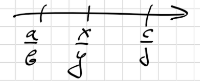
\includegraphics[width=30mm]{image2.png}

$\vspace{2 ex}$

$\dfrac{bx - ay}{by} = \dfrac{x}{y} - \dfrac{a}{b} \leq \dfrac{1}{bd} |\cdot bdy ; \hspace{2 ex} xbd - ady \leq y; \hspace{2 ex} d \leq (bx - ay)d < y $

$xbd \leq (ad+1)y ; \hspace{2 ex} y \geq \dfrac{xbd}{ad+1} ;\hspace{2 ex} cy - dx \geq 1$

$0 < \dfrac{c}{d} - \dfrac{x}{y} < \dfrac{1}{bd} ;\hspace{2 ex} 0< \dfrac{cy - dx}{dy} < \dfrac{1}{bd} (\dfrac{cy - dx}{dy} \leq \dfrac{1}{dy}); \hspace{2 ex} \dfrac{1}{dy} < \dfrac{1}{bd} ; b<y$

Следствие: $\alpha \in (\dfrac{a}{b};\dfrac{c}{d})$ и $dc - ad = 1 \rightarrow$ та из $(\dfrac{a}{b}, \dfrac{c}{d})$, кто ближе к $\alpha$ - наилучшее приближение.

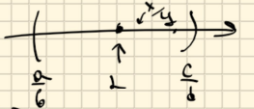
\includegraphics[width=30mm]{image3.png}

Следствие: $\dfrac{P_s}{Q_s} $ - наил. прибл к $\alpha$

$\dfrac{P_{s-1}}{Q_{s-1}}$ и $\dfrac{P_s}{Q_s} : P_{s-1} Q_s - P_s Q_{s-1}$


\subsection{Бесконечные цепные дроби}
$\alpha = [a_0,a_1,...,a_n,...] \vspace{1 ex}$

$ a_0 + \dfrac{1}{a_1 + \dfrac{1}{... + \dfrac{1}{a_n + \dfrac{1}{a_{n+1} + ...}}}} = \alpha$

$\eta_n = a_n + \dfrac{1}{a_{n + 1} + ...}$

$\eta_n = [a_n;a_{n+1}, a_{n+1}, ...] \rightarrow \alpha = [a_0;a_1,...,\eta_n]$

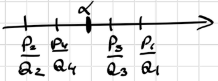
\includegraphics[width=30mm]{image.png}

\textbf{Утверждение} $\alpha$ между $\dfrac{P_s}{Q_s}$ и $\dfrac{P_{s+1}}{Q_{s+1}} $

Доказательство:

$\alpha = \dfrac{P_n}{Q_n} = \dfrac{\eta_n P_{n-1} + P_{n-2}}{\eta_n Q_{n-1} + Q_{n-2}} \vspace{2 ex}$

\begin{enumerate}
    \item
          $\alpha - \dfrac{P_{n-1}}{Q_{n-1}} = \dfrac{\eta_n P_{n-1} + P_{n-2}}{\eta_n Q_{n-1} + Q_{n-2}} - \dfrac{P_{n-1}}{Q_{n-1}}
              = \dfrac{\eta_n P_{n-1} Q_{n-1} + P_{n-2} Q_{n-1} - \eta_n P_{n-1} Q_{n-1} - P_{n-1} Q_{n-2}}{ Q_{n-1}(\eta_n Q_{n-1} + Q_{n-2})} =$

          $\dfrac{(-1)^{n-1}}{Q_{n-1}(\eta_n Q_{n-1} + Q_{n-2})}$

    \item $\alpha - \dfrac{P_{n-2}}{Q_{n-2}} = \dfrac{\eta_n P_{n-1} + P_{n-2}}{\eta_n Q_{n-1} + Q_{n-2}} - \dfrac{P_{n-2}}{Q_{n-2}}
              = \dfrac{\eta_n P_{n-1} Q_{n-2} + P_{n-2} Q_{n-2} - \eta_n P_{n-2} Q_{n-1} - P_{n-2} Q_{n-2}}{ Q_{n-2}(\eta_n Q_{n-1} + Q_{n-2})} = $

          $ = \dfrac{\eta_n (P_{n-1} Q_{n-2} - P_{n-2} Q_{n-1})}{Q_{n-2}(\eta_n Q_{n-1} + Q_{n-2}) }
              = \dfrac{\eta_n (-1)^{n-2}}{Q_{n-2}(\eta_n Q_{n-1} + Q_{n-2})}$

    \item $\left.\begin{array}{l}
                  \left|\alpha - \dfrac{P_{n-1}}{Q_{n-1}}\right| = \dfrac{Q_{n-2}}{\eta_n Q_{n-1}} \left|\alpha - \dfrac{P_{n-2}}{Q_{n-2}}\right| \\
                  \dfrac{Q_{n-2}}{\eta_n Q_{n-1}} < 1                                                                                             \\
                  Q_{n-2} < Q_{n-1} \leq \eta_n Q_{n-1}                                                                                           \\
              \end{array}\right|\Rightarrow \left|\alpha - \dfrac{P_{n-1}}{Q_{n-1}}\right| < \left|\alpha - \dfrac{P_{n-2}}{Q_{n-2}}\right|$
\end{enumerate}

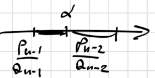
\includegraphics[width=30mm]{image1.png}
$\Rightarrow$ Следствие:$ |\alpha - \dfrac{P_{n}}{Q_{n}}| < \dfrac{1}{Q^2_n}$

Доказательство: $|\alpha - \dfrac{P_{n}}{Q_{n}}| \leq |\dfrac{P_{n+1}}{Q_{n+1}} - \dfrac{P_{n}}{Q_{n}}| = \dfrac{1}{Q_n Q_{n+1}} < \dfrac{1}{Q^2_n}  \vspace{2 ex}$

$Q_{n+1} > Q_n$

$\dfrac{1}{Q_{n+1}} < \dfrac{1}{Q_n} $

\subsection{Пример}
\subsubsection{Действие:}  ты берёшь и смотришь хмммм к какому числу $\sqrt{28}$ ближе СНИЗУ то есть $\sqrt{28}$ это примерно $5.xxxx$ значит пишем 5+ и 5- \par
$\sqrt{28} = 5 + (\sqrt{28} - 5)$\par
\subsubsection{Действие:} Мы переворачиваем дробь тупо берём и переворачиваем\par
$5 + \dfrac{1}{\dfrac{1}{\sqrt{28} - 5}}$
\subsubsection{Действие:}
Теперь мы домножаем на сопяжённые верхнюю и нижнюю чать, то есть $\dfrac{1 * (\sqrt{28} + 5)}{(\sqrt{28} - 5)(\sqrt{28} + 5)}$
(Надеюсь, все знают что такое сопряжённые и как на них домнажать)\par
$5 + \dfrac{1}{\dfrac{\sqrt{28}+5}{3}}$

\subsubsection{Действие:}
И последенее действиие после которого весь алгоритм зацикливается\par
Мы должны вынести целую часть то есть у нас есть $\dfrac{\sqrt{28}+5}{3}$ наверху у нас примерно получится $10.xxxxx$ значит мы выносим целую часть, которая равна 3 наверху у нас остаётся $1.xxxx$ и чтобы это получить из корня который равен $\sqrt{28} = 5.xxxx$ мы вычитаем $4$. Таким образом у нас получается\par
$5 + \dfrac{1}{3 + \dfrac{\sqrt{28} - 4}{3}}$
\subsubsection{Действие:}
Мы снова переварачиваем дробь и получаем уже\par
$5 + \dfrac{1}{3 + \dfrac{1}{\dfrac{3}{\sqrt{28}-4}}}$\par
\vspace{2 ex}
и опять домножаем на сопряжённые получаем\par
$5 + \dfrac{1}{3 + \dfrac{1}{\dfrac{3(\sqrt{28} + 4)}{12}}} = 5 + \dfrac{1}{3 + \dfrac{1}{\dfrac{\sqrt{28} + 4}{4}}}$\par
\vspace{2 ex}
Выносим целую часть\par
$5 + \dfrac{1}{3 + \dfrac{1}{2 + \dfrac{\sqrt{28} - 4}{4}}}$\par
\vspace{2 ex}
И так далее. Каждое целое число это значение в цепной дроби. Сейчас мы дошли до $[5;3,2]$. Продолжать можно пока не захотите остановиться или пока не начнётся уже период тогда уже нет смысла считать одно и тоже будет.

\section{Простые числа. Основная теорема арифметики.}
\subsection{Определение}
$p \in \mathbb{N}$ простое, если есть ровно 2 натуральных делителя.
\subsection{Определение}
$a \in \mathbb{N}$ составное, если есть $>2$ натуральных делителей
\subsection{Утверждение}
$p$ - простое, $ab$ $\vdots$ $p$ $\Rightarrow$ $a$ $\vdots$ $p$ или $b$ $\vdots$ $p$
\subsubsection{Доказательство}
Пусть $a$ не делится на $p$, НОД($a, p$) = 1 $\Rightarrow$ $b$ $\vdots$ $p$
\subsection{Утверждение}
$\gcd(a, bc) = 1 \Leftrightarrow \ \gcd(a, b) = 1$ и $\gcd(a, c) = 1$
\subsubsection{Доказательство}
$|=>|$ НОД($a, b$) = $d$ \par
$a$ $\vdots$ $d$ \par
$bc$ $\vdots$ $b$ $\vdots$ $d$ \par
НОД($a, bc$) $\vdots$ $d$ \par
$1$ $\vdots$ $d$ \par
$d$ = $1$\par
$|<=|$ НОД($a, bc) = d$\par
НОД($b, d) = f$ \par
$a$ $\vdots$ $d$ $\vdots$ $f$ \qquad  $a$ $\vdots$ $d$ $\vdots$ $\frac{d}{f}$ \par
$bc$ $\vdots$ $d$ \par
$b$ $\vdots$ $f$ \par
$c$ $\vdots$ $\frac{d}{f}$\par
НОД($a, b) \vdots f$ \par
$1$ $\vdots$ $f$ \qquad $\frac{d}{f}$ = $1$\par
$f = 1$ \qquad $d = 1$ \par
\subsection{Утверждение}
$\gcd(b, c) = 1$ \par
$a\ \vdots\ b,\ a\ \vdots\ c\ \Rightarrow\ a\ \vdots\ bc$
\subsubsection{Доказательство}
$a\ \vdots\ \text{НОК}(b, c) = \frac{bc}{\gcd(b, c)} = bc$
\subsection{Утверждение}
$\gcd(b, c) = 1\ \Rightarrow\ \gcd(a, bc) = \gcd(a, b)\gcd(a, c)$
\subsubsection{Доказательсто}
НОД(НОД(a, b), НОД(a, c)) = d \par
$b$ $\vdots$ НОД$(a, b)$ $\vdots$ $d$ \par
$c$ $\vdots$ НОД$(a, c)$ $\vdots$ $d$ \par
НОД$(b, c)$ $\vdots$ $d$ \par
$d = 1$\par
$bc$ $\vdots$ НОД$(a, b)$, $bc$ $\vdots$ НОД$(a, c)$ $\Rightarrow$ $bc$ $\vdots$ НОД$(a, b)$НОД$(a, c)$ \par
$f-$ОД$(a, bc)$ \qquad
$a$ $\vdots$ $f$ \qquad
$bc$ $\vdots$ $f$ \par
НОД$(a, b)$ $=$ $g$, НОД$(\frac{b}{g}, \frac{f}{g})$ $=$ $1$ \qquad $c$ $\vdots$ $\frac{f}{g}$\par
$a$ $\vdots$ $f$ $\vdots$ $g$ \qquad $b$ $\vdots$ $g$ \qquad НОД$(a, b)$ $\vdots$ $g$\par
$a$ $\vdots$ $f$ $\vdots$ $\frac{f}{g}$, $c$ $\vdots$ $\frac{f}{g}\Rightarrow$ НОД(a, c) $\vdots$ $\frac{f}{g}$\par
НОД$(a, b)$НОД$(a, c)$ $\vdots$ $f$
\subsection{Утверждение}
$\forall a \in \mathbb{N},\ a > 1 \Rightarrow \exists \ p$ простое $a\ \vdots \ p$
\subsubsection{Доказательство}
$1,d_1,..., d_k$ - делители a \par
$d_1$ простое $d_1 \ \vdots \ f$ \qquad $a \ \vdots \ d_1 \ \vdots \ f$ \par
\subsection{Утверждение(основная теорема арифметики)}
$\forall a \in \mathbb{N}, \ a>1, \qquad a = p_1^{\alpha_1} ... p_k^{\alpha_k}, \ \ \ \ \alpha_i = 0$
\subsubsection{Доказательство}
$a = a \qquad a=bc \qquad$ $a=bc=p_1^{\beta_1}...p_1^{\beta_1}p_3^{\beta_3}...p_k^{\beta_k}$ \par $a=p_1^{\alpha_k}...p_k^{\alpha_k} = q_1^{\beta_1}...q_l^{\beta_l}$ \par
$p_1 = q_1a=p_2^{\alpha_2}...p_n^{\alpha_n}=q_1^{\beta_1-2}...q_l^{\beta_l}$
\subsection{Утверждение}
$\alpha=p_1^{\gamma_1}...p_k^{\gamma_k} \qquad \beta=$ $p_1^{\delta_1}...p_k^{\delta_k}$\par
$\gamma_i \geq 0 \qquad \delta_i \geq 0 \qquad p_i -$ простое \par
НОД$(\alpha, \beta) =$
$ p_1^{min(\gamma_1, \delta_1)}...p_k^{min(\gamma_k, \delta_k)}$ \par
НОК$(\alpha, \beta)=\prod_{i=1}^kp_i^{max(\gamma_i, \delta_l)}$
\subsubsection{Доказательство}
$] d = \prod_{i=1}^k p_i^{min(\gamma_i, \gamma_i)}$ \par
$\alpha \ \vdots \ d, \  \beta \ \vdots \ d, \ ]d'-$ОД$(\alpha, \beta)$ \par
$\alpha \ \vdots \ q_1^{\epsilon_1}...q_s^{\epsilon_s}$ \par
$]| q_1 \not= p_1, \ q_1\not= p_2,...,q_1\not=p$ \par
$p_1^{\gamma_1}...p_k^{\gamma_k} \ \vdots \ q_1,$ НОД$(p_1^\gamma, q_1) = 1$
$\Rightarrow \ p_2^{\gamma_2}...p_k^{\gamma_k} \ \vdots \ q_1 \Rightarrow$
$p_k^{\gamma_k}\ \vdots \ q_1$ \par
$d' = p_1^{\epsilon_1}...p_k^{\epsilon_k}$ \par
$]| \epsilon_1>\gamma_1 \ \ \ \ \alpha \ \vdots \ d' \ \vdots \ p_1^{\epsilon_1} \ \ \ \ p_1^{\gamma_1} \ \vdots \ p_1^\epsilon$ \par
$p_1^{\gamma_1 - \epsilon} \in \mathbb{Z} \ \ \ \ \gamma_1-\epsilon \geq 0 \ \ \ \ \epsilon_1 \leq \gamma_1 \ \ \ \ \epsilon_1 \leq \delta_1 \ \ \ \ \epsilon_1 \leq min(\gamma_1, \delta_1) \ \ \ \ d' \leq d$ \par
НОД$(\alpha, \beta)$НОК$(\alpha, \beta) = \alpha\beta$ \par
НОК$(\alpha, \beta) = \frac{\alpha\beta}{gcd(\alpha, \beta)}=\prod_{i=1}^k \frac{p_i^{\gamma_i}p_i^{\delta_i}}{min(\gamma_i, \delta_i)}=\prod_{i = 1}^kp_i^{max(\gamma_i, \delta_i)}$
\subsubsection{Пример}
$24 = 2^3*3*5^0$ \par $90 = 2 * 3^2 *5$ \par
НОД$(24, 90) = 2^{min(3, 1)}3 ^{min(1, 2)}5^{min(0, 1)} = 2^1*3^1*5^0=6$

\section{Кольца вычетов. Полная система вычетов. Теорема о кольцах вычетов по простому модулю}
\subsection{Кольца вычетов}
$<x,+,*>$
\begin{equation*}
    \text{Кольцо}
    \begin{cases}
        \text{Абелева группа}
        \begin{cases}
            \text{Группа}
            \begin{cases}
                \text{Полугруппа}
                \begin{cases}
                    1^{\circ} \quad (a+b)+c = a+(b+c)
                \end{cases}
                \\
                2^{\circ} \quad \exists 0: a+0 = a
                \\
                3^{\circ} \quad \forall a \quad\exists (-a): a + (-a) = 0
            \end{cases}
            \\
            4^{\circ} \quad a + b = b + a
        \end{cases}
        \\
        5^{\circ} \quad \begin{cases}
                            (a+b)*c = (a*c) + (b*c)
                            \\
                            c*(a+b) = (c*a) + (c*b)
                        \end{cases}
    \end{cases}
\end{equation*}

\subsubsection{Свойства колец}
\begin{itemize}
    \item Кольцо ассоциативно: $(a*b)*c = a*(b*c)$
    \item Кольцо коммутативно: $a*b = b*a$
    \item Кольцо с единицей: $\exists 1: 1*a = a$
    \item Область целостности: $\exists a\ne 0, b \ne 0 \Rightarrow a*b \ne 0$
\end{itemize}

\subsubsection{Примеры колец}
\begin{itemize}
    \item Кольцо целых чисел $\mathbb{Z}$, кольцо рациональных чисел $\mathbb{Q}$, кольцо вещественных чисел $\mathbb{R}$
    \item Кольцо $\mathbb{Z}[i]$ целых гауссовых чисел вида $a + bi$, где $a,b \in \mathbb{Z}$
    \item Кольцо $\mathbb{Z}[\sqrt{2}]$ вещественных чисел вида $a + b\sqrt{2}$ c целыми $a,b$
\end{itemize}

\subsubsection{Поле}
Поле - коммутативное ассоциативное кольцо с единицей в котором $\forall a \ne 0 \quad \exists a^{-1}: a * (a^{-1}) = 1$

\subsubsection{Множество классов вычетов}
Множество классов вычетов (обозначают $\mathbb{Z}_m$) является ассоциативным коммутативным кольцом с единицей
\subsubsection{Примеры полей}
\begin{itemize}
    \item Числовые поля $\mathbb{Q}$, $\mathbb{R}$
    \item Поле $\mathbb{Q}[i]$ рациональных чисел вида $a + bi$, где $a,b \in \mathbb{Q}$
    \item Поле $\mathbb{Z}[\sqrt{2}]$ вещественных чисел вида $a + b\sqrt{2}$ c рациональными $a,b$
\end{itemize}

\subsection{Полная система вычетов}

Классом вычетов по модулю m называют множество чисел с одинаковым остатком при делении на m
\subsubsection{Определение}
Если взять по одному представителю из каждого класса вычетов, то эти m чисел образуют полную систему вычетов по модулю m

\subsubsection{Примеры простейших полных систем вычетов}
\begin{itemize}
    \item $\{0, 1, 2, \dots, m-1\}$ наименьшие положительные вычеты
    \item $\{0, -1, -2, \dots, -(m-1)\}$ наименьшие отрицательные вычеты
    \item для произвольного $a \in \mathbb{Z} \quad\{a, a+1, a+2, \dots, a+(m-1)\}$
    \item если $D(a,m) = 1$, то $\{0, a, 2a, \dots, (m-1)a\}$
\end{itemize}

\subsection{Теорема о кольцах вычетов по простому модулю}

Китайская теорема об остатках утверждает, что система сравнений с попарно взаимно простыми модулями
$m_1, m_2, \dots, m_k$:\\
\begin{equation*}
    \begin{cases}
        x \equiv c_1  (\text{mod } m_1) \\
        x \equiv c_2 (\text{mod } m_2)  \\
        \dots                           \\
        x \equiv c_k (\text{mod } m_k)
    \end{cases}
\end{equation*}
всегда разрешима и имеет единственное решение по модулю ($m_1m_2\dots m_k$)\\
\\
Другими словами, китайская теорема об остатках утверждает, что кольцо вычетов по модулю произведения нескольких попарно взаимно простых чисел является прямым произведением соответствующих множителям колец вычетов

\subsubsection{Теорема}
Если модуль $m$ - составное число, то $\mathbb{Z}_m$ не является полем\\
\\
Доказательство\\
\\
Пусть \quad $m = p_1p_2$, \qquad $1 < p_1, p_2 < m$\\
\\
Будем считать, что $P_1, P_2 \in \mathbb{Z}_m$ - классы вычетов, которым принадлежат $p_1, p_2$. Тогда:\\
\\
\quad $P_1P_2 = 0$, \quad $P_1, P_2 \ne 0$ \quad и элементы $P_1, P_2$ необратимы.\\
Почему $p_1$ и $p_2$ необратимы:\\
$\forall i \in [1, p_2) \qquad p_1 \cdot i < m, p_1 \neq 1$ \\
$p_1 * p_2 = 0 \neq 1$\\
$p_1 * (p_2 + 1) = p_1 (\mod m) \neq 1\ \Rightarrow$ у $p_1$ нет обратного \\
Следовательно, $\mathbb{Z}_m$ - не поле

\section{Линейные сравнения}
\textbf{Теорема:}
Если $\gcd(a, b) = d$, то уравнение $a*x\equiv b \pmod{m}$ имеет решение тогда и только тогда, когда $b \vdots d$.\\
\textbf{Доказательство} ---------------------------------------------------------

\vspace{0.3cm} %

$\Rightarrow$ $ax \equiv b \pmod{m}$, то $ax - b \vdots m \vdots d$, так как $ax \vdots d$ и $b \vdots d$.

$\Leftarrow$$\frac{a}{d}x \equiv \frac{b}{d} \pmod{\frac{m}{d}}$

$\gcd\left(\frac{a}{d}, \frac{b}{d}\right) = 1$ и $\left(\frac{a}{d}\right)^{\phi\left(\frac{m}{d}\right)} \equiv 1 \pmod{\frac{m}{d}}$.

    \vspace{0.5cm} %
$\left(\frac{a}{d}\right)^{\phi\left(\frac{m}{d}\right)} x \equiv \left(\frac{a}{d}\right)^{\phi\left(\frac{m}{d}\right) - 1} \frac{b}{d} \pmod{m}$

    \vspace{0.5cm} %
$x \equiv \left(\frac{a}{d}\right)^{\phi\left(\frac{m}{d}\right) - 1} \frac{b}{d} \pmod{\frac{m}{d}}$

    \vspace{0.5cm} %
$\left(\frac{a}{d}\right)^{\phi\left(\frac{m}{d}\right) - 1} \cdot \frac{b}{d} \equiv d \cdot \left(\frac{a}{d}\right)^{\phi\left(\frac{m}{d}\right)} \cdot \frac{b}{d} \pmod{m}= d\left[k\frac{m}{d} + 1\right]\frac{b}{d} = [km + d]\frac{b}{d} \equiv d\frac{b}{d} \pmod{m} = b$.

    \vspace{0.3cm} %
    --------------------------------------------------------------------------------

    \vspace{0.5cm} %
$1)
ax \equiv b \pmod{m} \\
\gcd(a, m) = 1 $! решение$ \Rightarrow x \equiv a^{\phi(m)-1}b \pmod{m}
$
    \vspace{0.5cm} %

$2)
\gcd(a, m) = d ;   b \vdots d  \\
\frac{a}{d} x \equiv \frac{b}{d} \pmod{\frac{m}{d}} \\
x \equiv \left(\frac{a}{d}\right)^{\phi\left(\frac{m}{d}\right) - 1} \frac{b}{d} \pmod{\frac{m}{d}}, \text{ где } \left(\frac{a}{d}\right)^{\phi\left(\frac{m}{d}\right) - 1} \frac{b}{d} = x_0
$
    \vspace{0.5cm} %

$d \text{ реш:}\left[ \begin{array}{l}
    x \equiv x_0 \pmod{m}               \\
    x \equiv x_0 + \frac{m}{d} \pmod{m} \\
    x \equiv x_0 + (d-1)\frac{m}{d} \pmod{m}
\end{array} \right.
$
    \vspace{0.5cm} %

$3)
\gcd(a, m) = d ; b \not\vdots d $   => $\emptyset  \\$

$4)
    ax \equiv b \pmod{m} \\$
$ax - b \vdots m$\\
$ax - b = my$\\
$b =ax- my$\\
$x=x_0+t\frac{m}{d}$\\

    \textbf{Утв:}
$p$-простое$ , a<p $\\
    Решение  $x\equiv \frac{C_p^a}{p}*b*(-1)^k \pmod{m}$,где k = a -1\\
    \textbf{Доказательство:}\\
$ C_p^a = \frac{p!}{a!(p-a)!}=\frac{p(p-1)....(p-a+1)}{1*2...a} $\\
$\frac{C_p^a}{p}= =\frac{p(p-1)....(p-a+1)}{1*2...(a-1)a}$\\
$(p-1)(p-2)...(p-a+1)\equiv (-1)(-2)....(-a+1) = (-1)^k*1*2....*(a-1)$,где k=a-1\\
$a\frac{C_p^a}{p}\equiv (-1)^k \pmod{p}$,где k=a-1\\
$ab\frac{C_p^a}{p} * (-1)^k\equiv b \pmod{p} $,где k=a-1\\
    \\
    \textbf{Теорема Критерий Вильсона}
    \\
$p$-простое $<=> (p-1)! \equiv -1 \pmod{p} $\\
    \textbf{Доказательство:}\\
$|=>|  (p-1)!= 1(p-1) $\\
$a^2 \equiv 1 \pmod{p}$\\
$a^2 -1 \vdots p$\\
$(a-1)(a+1) \vdots p$\\
    \\
$\left[ \begin{array}{l}
    a-1 \ \vdots\ p \\
    a+1 \ \vdots\ p \\
\end{array} \right.
$
    \\$\left[ \begin{array}{l}
        a \equiv 1 \pmod{p}  \\
        a \equiv -1 \pmod{p} \\
    \end{array} \right.
$
$|<=| p $- не простое $p = mn$\\
$(p-1)!\vdots m $\\
$(p-1)!\equiv -1 \pmod{p}$\\
$(p-1)!+1\vdots m\vdots p $\\

\textbf{Теорема Китайскаяя теорема об остатках}

$m_1,..,m_n $- попарно взаимно простые \\

$
    d \text{ имеет ! реш:}\left\{
    \begin{aligned}
        x \equiv C_1 \pmod{m1}         \\
        .............................. \\
        .............................. \\
        x \equiv C_n \pmod{m_n}        \\.
    \end{aligned}
    \right.
$\\
$x\equiv C\pmod{M} $, где$M = m_1,...m_n$\\

\textbf{Доказательство:}\\
$M_i=\frac{M}{m_i}$\\
\\
$\gcd(M_i, m_i) = 1 $\\
\\
$x*M_i\equiv 1\pmod{m_i} => x\equiv a_i\pmod{m_i} $\\
\\
$x = \sum_{i=1}^{n} M_i*a_i*C_i\equiv M_i*a_i*C_i\pmod{m_i}\equiv C_i\pmod{m_i} $\\
$|!| x \not\equiv y \pmod{M} $\\
$x\equiv C_i\pmod{m_i}\equiv y\pmod{m_i}$\\
$x-y\vdots m_i => x-y\vdots M$\\
$x = (C_1,...C_n)$-китайский код числа X\\
$y = (d_1,..d_n)$\\
$x+y = (C_1+d_1,...C_n+d_n)$

\setcounter{section}{7}

\section{Функция Эйлера и её свойства}

\subsection{Определение} Функция Эйлера $\varphi(n)$ ставит в соответствие каждому натуральному $n$ количество чисел, меньших $n$ и взаимно простых с $n$. Будем полагать $\varphi(1)=1$.

\subsection{Свойства}
\begin{enumerate}
    \item $p\in P:\varphi(p)=p-1,$ - Функция Эйлера для простого числа
    \item $p\in P:k\in N:\varphi(p^{k})=p^{k}-p^{k-1},$ - Функция Эйлера для простого числа в степени
    \item $\sqsupset$НОД$(a,b)=1=>\varphi(ab)=\varphi(a)\varphi(b)$, при $a,b\in \mathbb{N}$ - мультипликативность функции Эйлера
\end{enumerate}

\subsection{Утверждение} Для простого $p$ значение функции Эйлера задаётся формулой: \[\varphi(p)=p-1,\] которая следует из определения. Если $p$ - простое, то все числа, меньшие $p$, взаимно просты с ним, а их ровно $p-1$ штук.
\par Для вычисления функции Эйлера от степени простого числа используют следующую формулу: \[\varphi(p^{n})=p^{n}-p^{n-1}.\]
\par \textit{Доказательство.} Подсчитаем количество чисел от $1$ до $p^{n}$, которые не взаимно просты с $p^{n}$. Все они, очевидно, кратны $p$, то есть, имеют вид: $p,2p,3p,\dots,p^{n-1}p$. Всего таких чисел $p^{n-1}$. Поэтому количество чисел, взаимно простых с $p^{n}$, равно $p^{n}-p^{n-1}$.

\subsection{Следствие} Если НОД$(a,b)=1$, тогда $\varphi(ab)=\varphi(a)\varphi(b)$.
\par \textit{Доказательство.} В полной системе вычетов по модулю $a$ существует $\varphi(a)$ значений $x$, таких, что НОД$(a,x)=1$. Также и для полной системы вычетов по модулю $b$ существует $\varphi(b)$ значений $y$, таких, что НОД$(b,y)=1$. Следовательно, всего имеется $\varphi(a)\varphi(b)$ значений $z$, взаимно простых с $ab$. Но значения $z$ образуют полную систему вычетов по модулю $ab$, и чисел, взаимно простых с $ab$, в ней $\varphi(ab)$.

\subsubsection{Пример} Для иллюстрации доказательства следствия составлена таблица 1 величин (x,y) при $a=4$ и $b=5$. Возможные значения для x - числа $0,1,2,3$, возможные значения для y - числа $0,1,2,3,4$. Из них для $x$ имеется два значения (1 и 3) взаимно простых с a (так как $\varphi(4)=2$). Соответственно для $y$ также есть четыре значения (1,2,3 и 4) взаимно простых с b (так как $\varphi(5)=4$). Эти значения помещены в кружочки, как и соответствующие им значения $z=ay+bx$.
\par Выделенные значения $z$ дают 8 чисел, меньших 20 и взаимно простых с ним, Таким образом: \[\varphi(20)=\varphi(4)\varphi(5)=2*4=8.\]

\begin{table}[h!]
    \centering
    \begin{tabular}{|c|c|c|c|c|c|}
        \toprule
        \multicolumn{1}{|c|}{} & \multicolumn{5}{c|}{\textbf{y}}                                                                             \\
        \cmidrule(){2-6}
        \textbf{x}             & {0}                             & \textcircled{1}  & \textcircled{2}  & \textcircled{3}  & \textcircled{4}  \\
        \midrule
        0                      & 0                               & 4                & 8                & 12               & 16               \\
        \textcircled{1}        & 5                               & \textcircled{9}  & \textcircled{13} & \textcircled{17} & \textcircled{1}  \\
        2                      & 10                              & 14               & 18               & 2                & 6                \\
        \textcircled{3}        & 15                              & \textcircled{19} & \textcircled{3}  & \textcircled{7}  & \textcircled{11} \\
        \bottomrule
    \end{tabular}
    \caption{\textbf{Доказательство мультипликативности}}
\end{table}

\subsection{Следствие} Всякое натуральное число n>1 представляется в виде: \[n=p^{\alpha_{1}}_{1}*\dots*p^{\alpha_{k}}_{k},\] где $p_{1}<\dots<p_{k}$ - простые числа, $\alpha_{1}<\dots<\alpha_{k}$ - натуральные числа.
\par Тогда $\varphi(n)=p^{\alpha_{1}-1}_{1}(p_{1}-1)*p^{\alpha_{2}-1}_{2}(p_{2}-1)*\dots=n\biggl(1-\cfrac{1}{p_{1}}\biggl)*\biggl(1-\cfrac{1}{p_{2}}\biggl)$
\subsubsection{Пример} Для доказательства следствия приведён пример вычисления:

\begin{enumerate}
    \item $\varphi(49)=\varphi(7^{2})=7^{2}-7=42,$
    \item $\varphi(30)=\varphi(2*3*5)=\varphi(2)\varphi(3)\varphi(5)=(2-1)(3-1)(5-1)=8,$
    \item $\varphi(60)=60\biggl(1-\cfrac{1}{2}\biggl)*\biggl(1-\cfrac{1}{3}\biggl)*\biggl(1-\cfrac{1}{5}\biggl)=16.$
\end{enumerate}

\subsection{Следствие} Функция Эйлера $\varphi(n)$ принимает только чётные значения при $n>2$. Причём, если $n$ имеет $k$ различных нечётных простых делителей, то $2^{k}\mid\varphi(n)$.
\par \textit{Доказательство.} Если $\exists p>2$ и $p$ - простое число, тогда \[\varphi(n)\vdots(p-1)\vdots2.\] Тогда если $n=2^{k}$, то \[\varphi(n)=2^{k}\biggl(1-\cfrac{1}{2}\biggl)=2^{k-1}\vdots2.\]

\subsection{Теорема Формула Гаусса}
\subsection{Определение} Пусть d пробегает все делители числа m. Тогда \[m=\sum_{d\mid m}\varphi(d).\]
\par \textit{Доказательство.} $\sqsupset p$ - простое число. Тогда \[\varphi(p^{n})=p^{n-1}(p-1).\] Таким образом \[1+\varphi(p)+\varphi(p^{2})+\dots+\varphi(p^{\alpha})=1+(p-1)+\dots+(p^{\alpha}-p^{\alpha-1})=p^{\alpha}\] Пусть $m=p^{\alpha_{1}}_{1}*\dots*p^{\alpha_{k}}_{k}$, тогда \[\prod^{k}_{i=1}(1+\varphi(p_{i})+\dots+\varphi(p^{\alpha_{i}}_{i}))=\prod^{k}_{i=1}p^{\alpha_{i}}_{i}=m.\] Исходя из этого \[\prod^{k}_{i=1}\sum^{\alpha_{i}}_{j=0}\varphi(p^{j}_{i})=\sum_{\substack{
            0\leq j_{1}\leq \alpha_{1} \\
            \vdots \\
            0\leq j_{k}\leq \alpha_{k}
        }}\varphi(p^{j_{1}}_{1})*\varphi(p^{j_{2}}_{2})*\dots*\varphi(p^{j_{k}}_{k})=\sum_{\substack{
            0\leq j_{1}\leq \alpha_{1} \\
            \vdots \\
            0\leq j_{k}\leq \alpha_{k}
        }}\varphi(p^{j_{1}}_{1})*\dots*p^{j_{k}}_{k})=\sum_{d\mid m}\varphi(d)\]
\subsubsection{Пример} $\displaystyle\sum_{d\mid 30}\varphi(d)=\varphi(1)+\varphi(2)+\varphi(3)+\varphi(5)+\varphi(6)+\varphi(10)+\varphi(15)+\varphi(30)=1+1+2+4+2+4+8+8=30$

\subsection{Теорема Эйлера}
Пусть НОД$(a,m)=1$, тогда $a^{\varphi(m)}\equiv_{m}1.$
\par \textit{Доказательство.} Пусть НОД$(a,m)=1.$ Тогда классов вычетов взаимно простых с $m$ будет $\varphi(m)$. Пусть $\{x_{1},x_{2},\dots,x_{\varphi(m)}\}$ - представители классов, то $\{ax_{1},ax_{2},\dots,ax_{\varphi(m)}\}$ будут также взаимно просты с $m$. Также, если $ax_{i}\equiv_{m} ax_{j}$, то $x_{i}\equiv_{m} x_{j}.$ Следовательно, числа $ax_{i}$ - также представители классов вычетов, взаимно простых с $m$. Тогда каждое $ax_{i}$ сравнимо с одним и только одним $a_{j}$. \[x_{i}*\dots*x_{\varphi(m)}\equiv_{m} ax_{i}*\dots*ax_{\varphi(m)}.\] После сокращения получаем нужное сравнение: \[1\equiv_{m} a^{\varphi(m)}.\]

\subsection{Следствие: Малая теорема Ферма}
Если $p$ - простое число, то $a^{p}\equiv_{p}a$
\par \textit{Доказательство.}
\par Если НОД$(a,p)=1$, то $a^{\varphi(p)}\equiv_{p}1$, $a^{p-1}\equiv_{p}1$.
\par Если $a\vdots p$, то $a\equiv_{p}0$, $a^{p}\equiv_{p}a\equiv_{p}0$.

\subsection{Следствие}
Если p - простое число, то $(a+b)^{p}\equiv_{p}a^{p}+b^{p}$
\par \textit{Доказательство.} $(a+b)^{p}\equiv_{p}a+b\equiv_{p}a^{p}+b^{p}$

\subsection{Следствие}
Если
\begin{table}[h!]
    \begin{tabular}{r|c}
        $a\equiv_{m}b$                                     \\
        $c\equiv_{\varphi(m)}d$ & $=>a^{c}\equiv_{m}b^{d}$ \\
        НОД$(a,m)=1$
    \end{tabular}
\end{table}
\par \textit{Доказательство.} $a^{c}\equiv_{m}b^{c}\equiv_{m}b^{k\varphi(m)+d}=(b^{\varphi(m)})^{k}*b^{d}\equiv_{m}b^{d}$
\par $c\equiv_{\varphi(m)}d=>c=k\varphi(m)+d$
\par НОД$(a,m)=1=>$ НОД$(b,m)=1$
\par НОД$(a,m)=$ НОД$(a-\widetilde{k}m,m)$

\subsubsection{Пример}
$25^{11^{35}}\equiv_{34}(-9)^{3}=81*(-9)\equiv_{34}-13*9=-117\equiv_{34}19$
\par НОД$(25,34)=1$
\par $11^{35}\equiv_{16}11^{3}\equiv_{16}(-5)^{3}=-125\equiv_{16}3$
\par $\varphi(34)=34\biggl(1-\cfrac{1}{2}\biggl)*\biggl(1-\cfrac{1}{17}\biggl)=16$
\par НОД$(11,16)=1$
\par $\varphi(16)=8$
\par $35\equiv_{8}3$

\section{Система шифрования RSA}

\textbf{Определение 1}: Функция $f$ называется односторонней, если для любого $x$ существует эффективный алгоритм вычисления $f(x)$, но не существует эффективного алгоритма решения уравнения $f(x) = a$.

\textbf{Определение 2}: Функция $f_k(x)$ называется функцией с секретом, если для любого $k$ и $x$ существует эффективный алгоритм вычисления $f_k(x)$, такой что $f_k(x) = a$, но не существует эффективного алгоритма решения уравнения $f_k(x) = a$. Однако, если значение $k$ известно, то существует эффективный алгоритм решения уравнения $f_k(x) = a$.

RSA, разработанная Райвестом, Шамиром и Адлеманом, определяется функцией $f(x) = x^e \mod m$, где $m$ - произведение двух больших простых чисел $p$ и $q$. Для выбора открытого ключа $e$ необходимо выбрать число, взаимно простое с функцией Эйлера $\varphi(m) = (p-1)(q-1)$. Закрытый ключ $d$ находится из уравнения $e \cdot d \equiv 1 \mod \varphi(m)$.

Для шифрования сообщения $x$ отправитель (Алиса) использует открытый ключ $(m,e)$ получателя (Боба) и преобразует сообщение в зашифрованное сообщение $c$ с помощью формулы $c \equiv x^e \mod m$. Зашифрованное сообщение $c$ отправляется Бобу.

Для расшифровки сообщения Боб использует свой закрытый ключ $d$ и преобразует зашифрованное сообщение $c$ обратно в исходное сообщение $x$ с помощью формулы $x \equiv c^d \mod m$.

RSA также может использоваться для создания электронных подписей. Электронная подпись используется для подтверждения подлинности и целостности данных. Она создается путем хеширования сообщения и шифрования полученного хеша закрытым ключом отправителя. Получатель может проверить подлинность сообщения, расшифровав подпись с помощью открытого ключа отправителя и сравнив полученный хеш с хешем исходного сообщения.

P. S. $e$ в данном случае коэффициент, а не число Эйлера.

\section{Определение деления многочленов с остатком. Теорема Безу. Схема Горнера}
\subsection{Определение деления многочленов с остатком:}
\subsection{Определение:}
Для любых двух многочленов $f(x)$ и $g(x)$, $g(x)\neq {0}$ существуют $q(x)$ и $r(x)$, такие что: $f(x) = g(x)q(x) + r(x)$, при этом степень $r(x)$ строго меньше степени $g(x)$\par
\subsection{Свойства:}
\begin{itemize}
    \item $f(x) \ \vdots\ g(x)$, $g(x) \ \vdots\  h(x)$ $\Rightarrow$ $f(x) \ \vdots\ h(x)$
    \item $f(x) \ \vdots\ g(x)$, $g(x) \ \vdots\  h(x)$ $\Rightarrow$ $f(x){\pm}g(x) \ \vdots\ h(x)$
    \item $f(x) \ \vdots\ h(x)$ $\Rightarrow$ $f(x)g(x) \ \vdots\ h(x)$
    \item $f(x) \ \vdots\ c, c\neq{0}$
    \item $f(x) \ \vdots\ g(x)$ $\Rightarrow$ $f(x) \ \vdots\ cg(x), c\neq{0}$
\end{itemize}
\subsection{Теорема Безу:}
\subsubsection{Теорема:}
Остаток от деления многочлена $P(x)$ на $x-a$ равен значению многочлена $P(a)$
\subsubsection{Доказательство:}
$P(x) = (x − a)Q(x) + r$, следовательно, $P(a) = r$
\subsubsection{Следствие:}
$P(x) \vdots (x − a)$ $\Rightarrow$ $P(a) = 0$
\subsection{Схема Горнера:}
\subsubsection{Определение:}
$P(x) = a_{n}x^{n} + a_{n-1}x^{n-1} + ... + a_{1}x + a_{0}$\par
$P(x)=(x-b)Q(x) + r$\par
$Q(x) = C_{n-1}x^{n-1} + C_{n-2}x^{n-2} + ... + C_{1}x + C_{0}$\par
$a_{n}x^{n} + a_{n-1}x^{n-1} + ... + a_{1}x + a_{0} = (x-b)(C_{n-1}x^{n-1} + ... + C_{0}) + r$\par
$x^{n}: a_{n} = C_{n-1}$\par
$x^{n-1}: a_{n-1} = C_{n-2} - bC_{n-1}$\par
$x^{n-2}: a_{n-2} = C_{n-3} - bC_{n-2}$\par
$.$\par
$.$\par
$.$\par
$x: a_{1} = C_{0} - bC_{1}$\par
$x^{0}: a_{0} = r - bC_{0}$\par
$C_{n-1} = a_{n-1}$\par
$C_{i} = bC_{i+1} + a_{i+1}$\par
$.$\par
$.$\par
$.$\par
$r = bC_{0} + a_{0}$\par
\subsubsection{Пример:}
Найти остаток от деления $p(x) = x^{4} - 3x^{2} + x -5$ на $x-2$\par
$b=2$\par
$ $\par
\begin{tabular}{ |c|c|c|c|c|c| }
    \hline
    $a_{n}$ & $a_{4}$ & $a_{3}$ & $a_{2}$ & $a_{1}$ & $a_{0}$ \\
    \hline
    \hline
    $b$     & $C_{3}$ & $C_{2}$ & $C_{1}$ & $C_{0}$ & $r$     \\
    \hline
\end{tabular}\par
$ $\par
Далее подставив значения мы можем найти $C_{n-1} ... C{0}$ и $r$\par
$ $\par
\begin{tabular}{ |c|c|c|c|c|c| }
    \hline
    $a_{n}$ & $1$     & $0$     & $-3$    & $1$     & $-5$ \\
    \hline
    \hline
    $2$     & $C_{3}$ & $C_{2}$ & $C_{1}$ & $C_{0}$ & $r$  \\
    \hline
\end{tabular}\par
$ $\par
Используя формулу $C_{n-1} = b*C_{n-1}+a_{n-1},C_{n-1}=a_{n}$ получим\par
$ $\par
\begin{tabular}{ |c|c|c|c|c|c| }
    \hline
    $a_{n}$ & $1$ & $0$ & $-3$ & $1$ & $-5$ \\
    \hline
    \hline
    $2$     & $1$ & $2$ & $1$  & $3$ & $1$  \\
    \hline
\end{tabular}\par
Ответ $p(x) =(x_{3} + 2x_{2} + x +3)(x-2) + 1$

\setcounter{section}{10}
\section{Интерполяционная формула Лагранжа}

\subsection{Формула Лагранжа}
$L(x) = \sum_{i=0}^n y_i l_i(x)$


$l_i(x) = \frac{x-x_0}{x_i-x_0} \times \frac{x-x_1}{x_i-x_1} \times ... \times \frac{x-x_{i-1}}{x_i-x_{i-1}} \times \frac{x-x_{i+1}}{x_i-x_{i+1}}$

\subsection{Пример}
Найти многочлен $P(x)$ минимальной степени, используя формулу Лагранжа:

$P(-3) = -36$

$P(0) = -9$

$P(5) = -44$

Для удобства пронумеруем многочлены от 0 до 2, где $P_0(-3)$, $P_1(0)$, $P_2(5)$

$l_0(x) = \frac{x-x_1}{x_0-x_1} \times \frac{x-x_2}{x_0-x_2} = \frac{x-0}{-3-0} \times \frac{x-5}{-3-5} = \frac{x(x-5)}{(-3)*(-8)} = \frac{x(x-5)}{24}$

$l_1(x) = \frac{x-x_0}{x_1-x_0} \times \frac{x-x_2}{x_1-x_2} = \frac{x+3}{0+3} \times \frac{x-5}{0-5} = \frac{(x+3)(x-5)}{3*(-5)} = \frac{(x+3)(x-5)}{-15}$

$l_2(x) = \frac{x-x_0}{x_2-x_0} \times \frac{x-x_1}{x_2-x_1} = \frac{x+3}{5+3} \times \frac{x-0}{5-0} = \frac{x(x+3)}{5*8} = \frac{x(x+3)}{40}$

Обозначим многочлен минимальной степени $L(x)$:

$L(x) = -36\frac{x(x-5)}{24} + (-9)\frac{(x+3)(x+5)}{-15} + (-44)\frac{x(x+3)}{40}$

Чтобы найти многочлен минимальной степени, преобразуем многочлен к стандартному виду:

$L(x) = -\frac{3}{2}x(x-5) + \frac{3}{5}(x+3)(x-5) - \frac{11}{10}x(x+3) =$

$= -\frac{3}{2}(x^2-5x) + \frac{3}{5}(x^2+3x-5x-15) - \frac{11}{10}(x^2+3x) =$

$= -\frac{3}{2}x^2 + \frac{15}{2}x + \frac{3}{5}x^2 - \frac{6}{5}x - 9 - \frac{11}{10}x^2 - \frac{33}{10}x =$

$= \frac{-15+6-11}{10}x^2 + \frac{75-12-33}{10}x - 9 = -2x^2 + 3x - 9$

Итоговый вид многочлена: $L(x) = -2x^2 + 3x - 9$

\setcounter{section}{11}

\section{(Билет 12) Разложение многочленов на свободные от квадратов множетели.}
\subsection{Определение:}
\noindent Пусть K - поле
\\$P(x)\in K[x]$  \textbf{неприводим} if не $\exists$ нетривиальный делитель: не $\exists$ $Q(x) \in K[x]: 0 < deg(Q) < deg(P)$ и $ P(x) \vdots Q(x) $;
    \\$ P(x) \vdots  $ С
\\$ P(x) \vdots cP(x)$
    \\$x^2 - 2 $ над $\mathbb{Q}$
\\$\sqsupset\mid x^2-2 \vdots x - a$
    \\$a^2-2=0$
\\$a^2=2$
    \\$x^2-2=(x-\sqrt2)(x+\sqrt2)$
\\То есть
\\$x^2+1$ над $\mathbb{Q}$ \textbf{неприводим}!
    \\над $\mathbb{R}$ \textbf{неприводим}!
    \\$x^2+1=(x-i)(x+i)$ над $\mathbb{C}$
\\$x^2+1=(x^2+1)$ над $\mathbb{Z}$
    \subsection{Определение: $P(x)$ свободный от квадратов }
    \noindent не $\exists$ $ Q(x)$: $deg(Q) > 0$
    \\$ P(x) \vdots Q(x)^2 $
\\$ P(x) = {P_1(x)}{P_2(x)^2}{P_3(x)^3}$...${P_n(x)^n}$
    \\${P_1(x)}$,...,${P_n(x)}$ попарно взаимно/пр. и свободны от квадратов
\subsection{Утверждение: $P(x) = Q(x)^kM(x)$}
\noindent $\gcd(Q(x),M(x)) = 1$ и $Q(x)$ неприводим => $P'(x) = Q(x)^{k-1}N(x)$
\\$\gcd(Q(x),N(x)) = 1$
    \\ Доказательство:
    \\$P'(x) = kQ(x)^{x-1}Q'(x)M(x)+Q(x)M'(x)$
\\$P'(x) = Q(x)^{x-1}(kQ'(x)M(x)+Q(x)M'(x))$
    \\$kQ'(x)M(x)=N(x)- Q(x)M'(x) \vdots Q(x)$
\\$kQ'(x)\vdots Q(x)$ ?! Противоречие
    \\Это работает при $Z_k$ k характ поля, p - характ. k if $\forall a\in K a+a+...+a=0 $
    \\$K$-поле характеристики ноль
\subsection{Следствие:}
\noindent $P(x)=Q_1(x)^{k_1}$$... Q_m(x)^{k_n}$,$Q_i$- неприводимы => $P'(x)=Q_1(x)^{k_1-1}$$... Q_m(x)^{k_n-1}$,$Q$ вз./пр. с $Q_i$
\\Доказательство:
\\$P'(x)=\sum\limits _{i=1}^{m} K_iQ_1(x)^{k_1}$$...Q_m(x)^{k_n}$$Q'_i(x)=Q_1(x)^{k_1-1}$$...Q_m(x)^{k_m-1}$$\sum\limits _{i=1}^{n}\frac{k_iQ_1(x)...Q_m(x)}{Q_i(x)}Q'_i(x)$
    \\$\gcd(Q_1,Q_i)\neq 1$
\\$\gcd(Q_1,Q_i) = Q_i$
    \\$Q \vdots Q_i$
\\$Q(x)= k_1Q_2Q_3...Q_mQ'_1+k_2Q_1Q_3...Q_mQ'_2+...+...Q_{m-1}Q'_m\vdots Q_i$
    \\$k_iQ'_i\vdots Q_i$
\\$Q'_i\vdots Q_i =>$ Противоречие
    \subsection{Алгоритм разложения на свободные от  квадратов множ.:}
    \noindent На языке программирования питон:
    \\$j=1$
\\$while$ $deg P>0$
    \\\indent$p' = diff(P)$
    \\\indent$S=\gcd(P,P')$
    \\\indent$r = \dfrac{P}{S}$
    \\\indent$t = \gcd(r,P')$
    \\\indent$P_j=\dfrac{r}{t}$
    \\\indent$P=\dfrac{P}{r}$
    \\\indent$j+= 1$
    \\$return$ $P_1P^2_2...P_{j-1}$
\\
\\Где:
\\
\\$P=P_1P^2_2P^3_3...P^n_n$
    \\$P'=P_2P^2_3...P_n^{n-1}$
\\$\gcd(P,P')=P_2P_3^2...P_n^{n-1}$
    \\$r=\frac{P}{\gcd(P,P')}=P_1P_2...P_n$
\\$\gcd(r,P')=P_2...P_n$
    \\$\frac{r}{\gcd(r,P')}=P_1$
\\
\\Пример:
\\$P(x)=x^3+x^2-x-1$
    \\$P'(x)=3x^2+2x-1$
\\$\gcd(P(x),P'(x))=x+1=S(x)$
    \\$r(x)= P/S=x^2-1$
\\$\gcd(r,P')=x+1=t(x)$
    \\$P_1=x-1$
\\new $P=x+1$
\\$P'=1$
    \\$S=1$
\\$r = x+1$
    \\$t = 1$
\\$P_2=x+1$
    \\$P(x) = P_1(x)P_2(x)^2P_3(x)^3...P_n(x)^n$
\\$P_1(x),...,P_n(x)$ попарно вз./пр. и свободные от квадратов множетели
    \subsection{$P(x) \in\mathbb{Z} P(x)\vdots x - \frac{p}{q}\\NOD(p,q)=1 => a_n \vdots q $, где $p(v)=a_n(x^n)+...+a_0$}
    \subsection{Теорема Безу}
    \noindent $P(x) \vdots x - \frac{p}{q} => p(\frac{p}{q} = 0)$
    \\Доказательство:
    \\$\frac{a_nP^n}{q_n}+\frac{a_{n-1}P^{n-1}}{q^{n-1}}+\frac{a_1P}{q}+a_0=0$
\\$a_nP^n+a_{n-1}P^{n-1}q+...+a_nPq^{n-1}+a_0q^n=0$
    \\$a_np^n \vdots q => a_n \vdots q$
\\$a_0p^n \vdots p => a_0 \vdots q$
    \subsection{Критерий Эйзенштейна}
    \noindent $P(x) \in \mathbb{Z}[x]$
    \\$P(x) = a_nx^n+...+a_0$
\\$a_{n-1}\vdots P, a_{n-2} \vdots P,...,a_0\vdots P$ и $a_n$не$\vdots P=>$ $P(x)$ неприводим над $Q$
    \\Доказательство:
    \\Пусть $P(x) = f(x)g(x)$
    \\$f(x) = b_mx^m+...+b_0$
\\$g(x) = C_{n-m}x^{n-m}+...+C_0$
    \\$P(x) = a_nx^n+...+a_0=(b_mx^n+...+b_0)(C_{n-m}x^{n-m}+...+C_0)$
\\$a_0=b_0C_0 \qquad b_0 \vdots P$
    \\$. \hspace{6em}C_0$ не$ \vdots P$
\\$a_1=b_0C_2+b_1C_1+b_2C_0 => b_2\vdots P $
    \\$a_m=b_nC_m+...+b_mC_0 => b_{n-1}\vdots P $

\setcounter{section}{12}
\section{Неприводимые многочлены. Поля Галуа}
\subsection{Неприводимые многочлены}
\subsubsection{Определение}
Пусть $K$ — поле. Тогда $P(x) \in K[x]$ неприводим, если не существует нетривиальный делитель $Q(x) \in K[x]$, такой, что его степень больше 0, меньше степени многочлена $P$ и $P(x)$ делится на $Q(x)$:
\[
    \nexists Q(x) \in K[x] : 0 < \deg Q < \deg P \text{ и } P(x) \vdots Q(x)
\]
\subsubsection{Определение}
$P(x)$ свободный от квадратов, если не существует $Q(x)$, такой, что $\deg Q >$ и $P(x) \vdots Q^2(x)$.
\subsubsection{Утверждение}
$
    \begin{aligned}
         & P(x) = Q^k(x)M(x)                                                                             \\
         & \gcd(Q(x), M(X)) = 1 \text{ и } Q(x) \text{ неприводим } \Rightarrow P'(x) = Q^{k - 1}(x)N(x) \\
         & \gcd(Q(x), N(x)) = 1
    \end{aligned}
$
\subsubsection{Доказательство}
$
    \begin{aligned}
         & P'(x) = kQ^{k - 1}(x)Q'(x)M(x) + Q^k(x)M'(x)                                             \\
         & P'(x) = Q^{k - 1}(x)(kQ'(x)M(x) + Q(x)M'(x)) \text{, где } kQ'(x)M(x) + Q(x)M'(x) = N(x) \\
         & kQ'(x)M(x) = N(x) - Q(x)M'(x)\ \vdots\ Q(x)                                              \\
         & kQ'(x) \ \vdots\ Q(x) \text{ — противоречие}                                             \\
         & \deg Q' = \deg Q - 1                                                                     \\
    \end{aligned}
$

Это работает при $\mathbb{Z}_k$ ($k \not \vdots$  характериситку поля).

\subsubsection{Следствие}
$P(x) = Q_1^{k_1}(x)...Q_m^{k_m}(x)$, $Q_i$ — неприводимы $\Rightarrow\ P'(x) = Q_1^{k_1-1}(x)...Q_m^{k_m - 1}Q(x)$, $Q$ взаимно прост с $Q_i$
\subsubsection{Критерий Эйзенштейна}
$
    \begin{aligned}
         & P(x) \in \mathbb{Z}[x]                                                                                                            \\
         & P(x) = a_nx^n + ... + a_0                                                                                                         \\
         & a_{n-1} \vdots p,\ a_{n - 2} \vdots p,\ ..., a_0 \vdots p,\ a_n \not \vdots p \Rightarrow P(x) \text{ неприводим над } \mathbb{Q}
    \end{aligned}
$
\subsubsection{Доказательство}
Рассмотрим $P(x) = f(x)g(x)$.
\allowdisplaybreaks[4]
\begin{align*}
     & f(x) = b_mx^m + ... + b_0                                                              \\
     & g(x) = c_{n - m}x^{n - m} + ... + c_0                                                  \\
     & p(x) = a_nx^n + ... + a_0 = (b_mx^m + ... + b_0)\cdot(c_{n - m} x^{n - m} + ... + c_0) \\
     & a_0 = b_0c_0\ \vdots\ p \qquad b_0\ \vdots\ p \qquad c_0 \not\vdots\ \ p               \\
     & a_1 = b_0c_2 + b_1c_1 + b_2c_0\ \vdots\ p \Rightarrow b_2\ \vdots\ p                   \\
     & \vdots                                                                                 \\
     & a_m = b_0c_m + ... + b_mc_0\ \vdots\ p \Rightarrow b_{m - 1}\ \vdots\ p                \\
     & a_n = b_nc_{n - m}\ \vdots\ p \text{ — противоречие}                                   \\
\end{align*}
\subsection{Поля Галуа}
\subsubsection{Определение}
Конечное поле, или поле Галуа в общей алгебре — поле, состоящее из конечного числа элементов. Обозначается $\mathbb{F}_q$ или $\mathbf{GF}(q)$ или $<\mathbf{GF}(q), +, *>$, где $q = |\mathbf{GF}(q)|$ — порядок поля. Порядком поля называется количество входящих в него элементов. Пример: $\mathbb{Z}_p,\ p \in \mathbb{P}$.
\subsubsection{Определение}
Характериситка поля $F$ — наименьшее $n$, такое, что $\forall a \in F$ выполняется следующее равенство:
\[
    \underbrace{a + a + ... + a}_{n\text{ раз}} = 0
\]

Если такого $n$ не существует, то $n$ считается равным $0$.

\subsubsection{Лемма}
Характериситка поля — простое или $0$.
\subsubsection{Доказательство}
Рассмотрим $n = \alpha \beta$.
\[
    \underbrace{1 + 1 + ... + 1}_{n \text{ раз}} = 0
\]
\[
    \underbrace{\underbrace{1 + 1 + ... + 1}_{\alpha \text{ раз}} + \underbrace{1 + 1 + ... + 1}_{\alpha \text{ раз}} + ... + \underbrace{1 + 1 + ... + 1}_{\alpha \text{ раз}}}_{\beta \text{ раз}} = 0
\]
\[
    \underbrace{\alpha + \alpha + ... + \alpha}_{\beta \text{ раз}} = 0 \qquad \Rightarrow \text{ характеристика — } \mathbb{P}
\]
\subsubsection{Свойства}
$f(x) \in \mathbb{Z}_p[x]$ ($f(x)$ принадлежит множеству многочленов с целыми коэффициентами по модулю $p$)  $\mathbb{Z}_p[x] / f(x)$ (кольцо вычетов многочленов с целыми коэффициентами по модулю $f(x)$)

$
    \displaystyle
    \left.\begin{aligned}
         & g_1(x) \equiv_{f(x)} h_1(x) \\
         & g_2(x) \equiv_{f(x)} h_2(x) \\
    \end{aligned}\right| \Rightarrow \begin{aligned}
         & g_1 + g_2 \equiv_{f(x)} h_1 + h_2 \\
         & g_1g_2 \equiv_{f(x)} h_1h_2       \\
    \end{aligned}
$
\subsubsection{Теорема}
$\mathbb{Z}_p[x] / f(x)\ \Leftrightarrow\ f(x)$ неприводим над $\mathbb{Z}_p$.

$\deg f = m$    $\mathbf{GF}(p^m)$
\subsubsection{Доказательство}
\textbf{Прямое.} Рассмотрим $f(x) = g(x)h(x)$ \\
$g(x)h(x) \equiv_{f(x)} 0 \qquad | \cdot g^{-1}(x) $ \\
$h(x) \equiv_{f(x)} 0 |\Rightarrow f(x) = 0$

\textbf{От обратного.} $\forall g(x) \neq 0$ $\deg g < \deg p$ \\
$\gcd(g(x), f(x)) = 1\ \Rightarrow$ по расширенному алгоритму Евклида:\\
$a(x)g(x) + b(x)f(x) = 1$ \\
$a(x)g(x) \equiv_{f(x)} 1\ \Rightarrow\ a = g^{-1} \ \Rightarrow\ \mathbb{Z}_p$ — поле

\subsubsection{Связь с линейным пространством}
Поле Галуа образует линейное (векторное) пространство. Его аксиомы:
\begin{itemize}
    \item $(a + b) + c = a + (b + c)$
    \item $\exists 0 : a + 0 = a$
    \item $\forall a \  \exists(-a) : a + (-a) = 0$
    \item $a + b = b + a$
    \item $\alpha(a + b) = \alpha a + \alpha b$
    \item $(\alpha + \beta)a = \alpha a + \beta a$
    \item $\alpha(\beta a) = (\alpha \beta) a$
    \item $\exists 1 : 1 \cdot a = a$
\end{itemize}

$\alpha, \beta \in \mathbb{Z}_p$, $F$ — линейное пространство. $m = \dim F$.

\subsubsection{Определение}
$\alpha$ — примитивный элемент, если $\forall b \neq 0 \in F$ \qquad $b = \alpha^i$.

\section{Кодирование с исправлением ошибок. Граница Хэмминга. Полиномиальное кодирование}
\subsection{Кодирование с исправлением ошибок. Граница Хэмминга}
$d:M\times M \rightarrow \mathbb{R}$ - функция расстояния
\begin{enumerate}
    \item $d(a,b) \geq 0; \hspace{4 mm} d(a,b) = 0 \Leftrightarrow a = b$
    \item $d(a,b) = d(b,a)$
    \item $d(a,b) + d(b,c) \geq d(a,c)$
\end{enumerate}\par
$M = \mathbb{Z}_2^m$\par
$a \in M, \,a = (a_0, a_1, ..., a_{m-1})$\par
$d(a,b) = \sum\limits_{i=0}^{m-1} |a_i - b_i|$ - кодовое расстояние Хэмминга (КХР)\par
$a \bigoplus b = (a_0 \bigoplus b_0, ... , a_{m-1} \bigoplus b_{m-1})$\par
$ $\par
Теорема КРХ - формула расстояния на $\mathbb{Z}_2^m$\par
$d(a,b)+d(b,c) = \sum\limits_{i=0}^{n-1}|a_i - b_i|+\sum\limits_{i=0}^{n-1}|b_i - c_i|=\sum\limits_{i=0}^{n-1}(|a_i - b_i|+|b_i - c_i|) \geq \sum\limits_{i=0}^{n-1}|a_i - b_i + b_i - c_i| =$\par
$ =\sum\limits_{i=0}^{n-1}|a_i - c_i| = d(a,c)$\par
$A=\{a^{(0)}, a^{(1)}, ... , a^{(k)}\} \leq \mathbb{Z}_2^m$\par
$\hspace{1 cm} \uparrow$\par
\textit{кодовое слово}\par
$ $\par
Теорема. Если $\forall i \neq j$\par
$d(a^{(i)},a^{(j)} \geq 2r+1 \Rightarrow$ можно исправить $\leq r$ ошибок \par
$ $\par
\textit{Доказательство:} $a \in \mathbb{Z}_2^m$\par
$A_i = \{ b / d(a^{(i)}, b) \leq r \}$\par
$\sqsupset | \, A_i \cap A_j = \{ c \}$\par
\begin{tabular}{c|cc}
    $c \subset A_i$ &               & $d(c,a^{(i)}) \leq r$ \\
                    & $\Rightarrow$                         \\
    $c \subset A_j$ &               & $d(c,a^{(j)}) \leq r$ \\
\end{tabular}\par
$ $\par
$d(a^{(i)},a^{(j)}) \leq d(a^{(j)},c) + d(c,a^{(i)}) \leq 2r \hspace{4 mm} ?!$\par
$A_i$ - область декодирвоания $a^{(i)}$\par
$a^{(i)}+e \hspace{4 mm} d(a^{(i)}+e, a^{(j)}) \leq r \, | \Rightarrow a^{(i)}+e \in A_i \, | \Rightarrow$ декодирование однознач.\par
$|A_i| = 1 + C_m^1 + C_m^2 + ... + C_m^r \hspace{1 cm} |\mathbb{Z}_2^m| = 2^m$\par
$\sum\limits_{i=0}^{n-1}|A_i| \leq |\mathbb{Z}_2^m|; \hspace{1 cm} k = |A| \hspace{1 cm} k|A_i| \leq |\mathbb{Z}_2^m| \, |\Rightarrow k = \frac{2^m}{\sum\limits_{i=0}^{r} C_m^i}$ - граница Хэмминга\par
$M = \{ 0, 1 \} \, |\to A = \{ 000,...,111 \}$\par
$m = 3 \Rightarrow r = 1 \hspace{1 cm} d(a^0, a^1)=3 \geq 2r+1 \hspace{1 cm} k \leq \frac{2^3}{C_3^0 + C_3^1} = \frac{8}{1+3} = 2$\par
\textbf{Определение.} Код называется совершенным (или плотно упакованным), если $\bigcup\limits_{i=0}^{n-1}A_i = \mathbb{Z}_2^m$\par

\subsection{Полиномиальное кодирование}
$M \Rightarrow \widetilde{M}$\par
$M \to C \Rightarrow \widetilde{C} \to M$\par
$\uparrow \hspace{1 cm}$ $\uparrow$\par
\textit{сообщ.} \textit{код. слово}\par
Код линейный if $\, \forall a,b \in A$\par
Вес Хэмминга$\, W(a)$\par
$a \in A \leq \mathbb{Z}_2^m$\par
$a = (a_0,...,a_{m-1})$\par
$W(a) =$ количество ненулевых $a_i$\par
Минимальное кодовое расстояние $d^* = \overset{}{\underset{i \neq j}{min}} \, d(a^{(i)},a^{(j)})$\par
Лемма. $d^* = \overset{}{\underset{a \neq 0}{min}} \, W(a)$\par
\textit{Доказательство:} $\, W(a) = d(a,0) \geq d^*$\par
$d(a,b) = d(a+b,b+b) = d(a+b, 0) = W(a+b)$\par
$d^* = \overset{}{\underset{a \neq b}{min}} \, d(a,b) = \overset{}{\underset{a \neq b}{min}} \, W(a+b) = \overset{}{\underset{a \neq 0}{min} \, W(a)}$\par
$a = (a_0, a_1, ..., a_{m-1}) \, |\to a_0+a_1k+...+a_{m-1}x^{m-1}$\par
$ $\par
Код циклический\par
$if (a_0,a_1,...,a_{m-1}) \in A \Rightarrow (a_{m-1},...,a_{m-2}) \in A$\par
\begin{tabular}{cccc}
    $a \to A(x)$                                                                                             \\
                                                     & $a+b \to A(x) + B(x)$                                 \\
    $b \to B(x)$                                                                                             \\
    \\
    $a \to a_0 +a_1 x +...+ a_{m-1}x^{m-1}$          &                       & $xA(x) \, mod(x^m + 1)$       \\
    $a_2 \to a_{m-1} + a_0 x + ... + a_{m-2}x^{m-1}$ &                       & $x^m \equiv 1 \, mod(x^m +1)$ \\
\end{tabular}\par
$ $\par
$A(x)$ - количество кодов $\Rightarrow P(x)A(x)$ - кодов\par
Порождающий многочлен - ненулевое приведение мн. наименьшей степени в коде.\par
$A = \{ ... \}$\par
$ $\par
Теорема. $G(x)$ - порождающий многочлен\par
минимальный цикл кода $\Leftrightarrow x^m + 1 \ \vdots\  G(x)$\par
\textit{Доказательство:}\par
$\Leftarrow \, x^m+1 \ \vdots\  G(x)$\par
$A(x),B(x)$\par
$A=\{ P(x)G(x) \, mod(x^m +1 )\}$\par
\begin{tabular}{ccc}
    $A(x) = P_A(x)G(x)$ &  & $A(x)+B(x) = (P_A(x)+P_B(x))G(x)$   \\
    $B(x) = P_B(x)G(x)$ &  & $\alpha A(x) = (\alpha P_A(x))G(x)$ \\
\end{tabular}\par
$ $\par
$xA(x) \, mod(x^m+1)$\par
$xA(x) = xP_A(x)G(x)$\par
$ $\par
$r(x) = xA(x) \equiv _{x^m+1} Q(x)G(x)+R(x)$\par
$xA(x) = S(x)(x^m+1)+r(x)=S(x)(x^n+1)+Q(x)G(x)+R(x)$\par
$P(x)G(x)=Q(x)(x^m+1)+R(x)$\par
$ $\par
\begin{tabular}{ccc}
    $P(x)G(x) \, mod(x^m+1)$ & $0 \equiv _{(x^m+1)}Q(x)G(x)+R(x)$ \\
    $x^m+1 \ \vdots\  G(x)$  & $degR < deg G \, ?! \Rightarrow$   \\
    $x^m+1 = Q(x)G(x)+R(x)$  & \textit{обязательно делится}       \\
\end{tabular}\par
$ $\par
$x^m+1$\par
$G(x)$\par
$d^* = \overset{}{\underset{P(x) \neq 0}{min}} \, W(P(x)G(x) \, mod x^m+1)$\par
$d^* > 2r+1 \hspace{2 cm} r < \frac{d^*}{2}$\par
$ $\par
$M \to C$\par
$M(x) \to C(x)$\par
$C(x) = M(x)G(x)$\par
$C(x)+E(x)$\par
$\widetilde{C}(x)= C(x)+E(x)$ - многочлен ошибок\par
\textit{$W(E(x)) \leq r$}\par
$\widetilde{C}(x) \, mod(G(x))=S(x)$ - синдром \par
$ $\par
Теорема. $E_1(x) \neq E_2(x) \Rightarrow E_1(x) \, mod G(x) \neq E_2(x) \, mod G(x)$\par
$W(E_1(x)) \leq r$\par
$W(E_2(x)) \leq r$\par
$ $\par
\textit{Доказательство:}\par
$E_1(x) + E_2(x) \neq 0$\par
$W(E_1(x)+E_2(x)) \leq 2r$\par
$ $\par
$\sqsupset E_1(x) \equiv E_2(x) \, mod G(x)$\par
$E_1(x)+E_2(x) \ \vdots\  G(x), \, W(E_1+E_2) \geq d^* \geq 2r+1$\par
$\widetilde{C}(x)=C(x)+E(x) = M(x)G(x)+E(x)$\par
$mod G(x):$\par
$\hspace{1 cm} S(x) \equiv E(x), \, C(x) = \widetilde{C}+E(x)$\par
$\hspace{1 cm} M(x) = \frac{C}{G}$\par
Если все ошибки в $deg G$ послед.  разр.\par
$x^i S(x) \equiv_{G(x)}T(x)$\par
$i \in [0;m-1]$\par
$W(T(x)) \leq r$\par
$x^mS(x) \equiv_{G(x)} x^{m-i}T(x)$\par
$\hspace{5 mm} |||$\par
$x^m+1 \equiv_{G(x)}0$\par
$ $\par
Теорема. $G(x) \ \vdots\  x+1 \geq W(P(x)G(x)) \ \vdots\  2$\par
$ $\par
\textit{Доказательство:} $\, G(x) = (x+1)A(x)$\par
$P(x)G(x) \ \vdots\  x+1$\par
$P(1)G(1) = 0$\par
$W(P(x)G(x)) \ \vdots\  2$\par
$ $\par
Следствие. $G(x) \ \vdots\  x+1 \geq$ детект. $\forall$ на ошиб.\par
$C(x)+E(x)$\par
\section{15. Префиксные коды.Неравенство Крафта.Алгоритм Хаффмана.}
\subsection{Префиксные коды}
$A = {a_1, \dots, a_n}$ - алфавит $ n \leq2^k\rightarrow$
$\begin{cases}
        a_1  \sim \underbrace{0\dots0}_{\text{k}} - c_1  \\
        a_2  \sim \underbrace{0\dots0}_{\text{k}}1 - c_2 \\
        \dots
    \end{cases}$
\newline$l_1=l_2=l_k$ ; $M:a_{i_1},a_{i_2},\dots,a_{i_s}$ ; $\alpha=ks\geq s\log{n}$

\textbf{Шеннон-Фано}

aabc

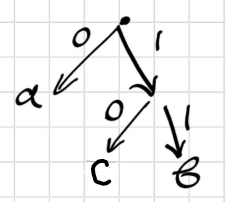
\includegraphics[width=20mm]{images/tree1.png}

$\underbrace{0}_{\text{a}}\underbrace{0}_{\text{a}}\underbrace{11}_{\text{b}}\underbrace{01}_{\text{c}}$

$\begin{cases}
        a  \sim 0  \\
        b  \sim 11 \\
        c \sim 01
    \end{cases}$

\subsubsection{Определение}
Код называется \textit{префиксным}, если ни одно кодовое слово не является началом другого кодового слова.

\subsection{Неравенство Крафта}
Для префиксного кода с длинами $l_1,\dots,l_s$

$\sum\limits_{i=1}^s 2^{-l_i} \leq 1$
\subsubsection{Доказательство}
$l_1\leq l_2 \leq \dots \leq l_s=q$

$A_i=\{\underbrace{(\dots)}_{\text{q двоичных чисел}})|$нач. с $l_i\}$

$A_i\cap A_j=\emptyset$

\subsubsection{Замечание}
$\cup A_i \leq \{ \underbrace{(\dots)}_{\text{q раз p}}\}$

$\sum\limits_{i=1}^s 2^{q-l_i} \leq 2^q$
\subsubsection{Теорема}
$p_1,\dots, p_n$ - вер, с которой встречаются $a_1, \dots, a_n$

Сред. длин. код. слова $L = \sum\limits_{i=1}^n l_ip_i $ ; $L \geq H(p_1, \dots, p_s)$
\subsubsection{Доказательство}
$\sqsupset q_i=\frac{2^{-l_i}}{\sum\limits_{i=1}^n2^{l_i}}$ ; $L-H(p_1,\dots, p_n)=\sum\limits_{i=1}^nl_ip_i+\sum\limits_{i=1}^np_i\log\limits_2{p_i}=\sum\limits_{i=1}^np_i\log\limits_2(p_i2^{l_i})=$

$=\sum\limits_{i=1}^np_ilog{\frac{p_i}{2^{-l_i}}} \geq \sum\limits_{i=1}^np_i\log\limits_2{\frac{p_i\sum\limits_{j=1}^n2^{-l_j}}{2^{-l_i}}}=\sum\limits_{i=1}^np_i\log\limits_2{\frac{p_i}{q_i}}=D(p||q) \geq 0$

$\rightarrow L \geq H(p_1, \dots, p_n) + D(p||q)$
\subsection{Алгоритм Хаффмана}

$a_1, \dots, a_n$ c $p_1, \dots, p_n$

$p_i = \frac{N(a_i)}{N}$

$p_1, p_2, \dots, p_s$

$p_i \geq p_j \rightarrow l_i \leq l_j$

$\sum\limits_{i=1}^s 2^{-l_i} \leq 1 (*)$

$p_{n-1}, p_n$ - наим.вер $\rightarrow l_{n-1} = l_n$

[чтобы знам $(*)$ сокращался]
\subsubsection{Пример}
$\underbrace{a \sim 0,22 \text{ ; }b \sim 0,2}_{ab \sim 0,42}$ ; $c \sim 0,15$; $\underbrace{d \sim 0,13 \text{ ; }e \sim 0,12}_{de \sim 0,25}$ ; $\underbrace{f \sim 0,1\text{ ; } g \sim 0,18 }_{fg \sim 0,18}$

$\underbrace{cfg \sim 0,33 \text{ ; }de \sim 0,25}_{cdefg \sim 0,58}$ ; $ab \sim 0,42$

$\underbrace{ab \sim 0,42 \text{ ; }cdefg \sim 0,58}_{abcdefg \sim 1}$

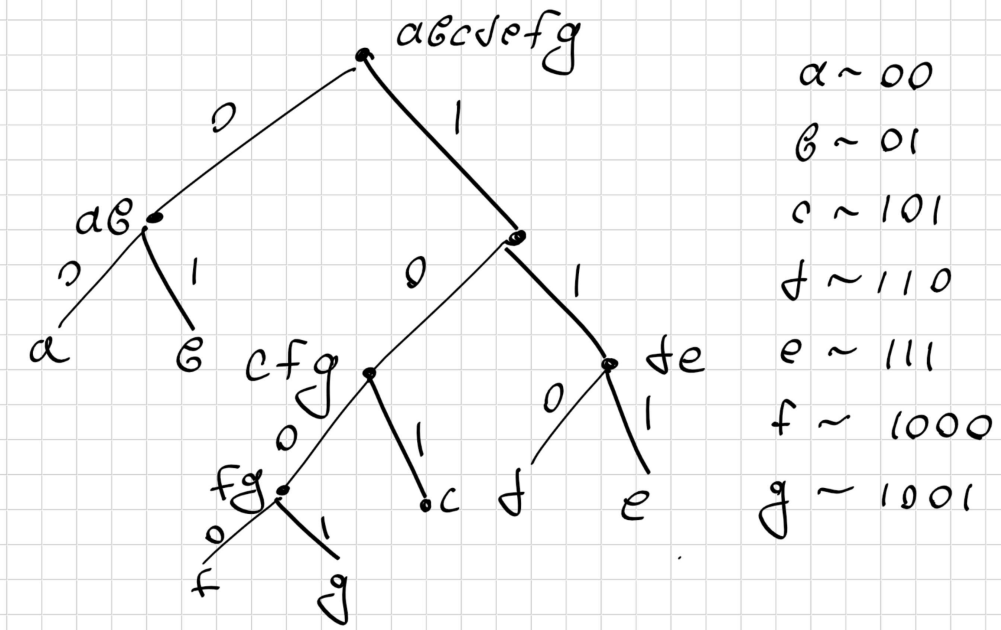
\includegraphics[width=100mm]{images/tree2.png}

\section{Коды Рида-Соломона:}
Рассмотрим алгоритм на примере:\par
Поле $GF(16)$ порождается присоединением к $GF(2)$ корня $a$ многочлена $P(x)$, $P(x) = x^{4}+x^{3}+1$\par
Пусть порождающий много член имеет вид $G(x) = (x-a)(x-a^2)(x-a^3)(x-a^4)$, тогда количество\par
ошибок многочлена которое исправит код Рида-Соломона $2t = deg(G(x)) \Rightarrow t = 4/2 = 2.$\par
Принятое сообщение $S(x) = a^{9}x^14 + a^5x^{13} + a^{12}x^{12} + a^{10}x^{11} + a^7x^9 + a^5x^8 + a^7x^7 + a^{13}x^6 + a^3x^5 +$\par $+ a^{11}x^4 + a^3x^3 + a^{10}x^2 + a^8x + a$\par
Вырази все $a$ пока они не зациклятся, т.е. $a_{n} = a_{0}$\par
$a^{0} = a^{0} = 1$\par
$a^{1} = a$\par
$a^{2} = a^2$\par
$a^{3} = a^3$\par
$a^{4} = a^3+1$\par
$a^{5} = a*a^{4} = a^{4}+a = a^3 + a +1$\par
$a^{6} = a^{3} + a^{2} + a + 1$\par
$a^{7} = a^2 + a + 1$\par
$a^{8} = a^3 + a^2 + a$\par
$a^{9} = a^2 + 1$\par
$a^{10} = a^3 + a$\par
$a^{11} = a^3 + a^2 +1$\par
$a^{12} = a + 1$\par
$a^{13} = a^2 + a$\par
$a^{14} = a^3 + a^2$\par
$a^{15} = a^4 + a^3 = 1$\par
И так как у нас поле $GF(16)$ то $a^{15} = a^{0} = 1$\par
Из порождающего многочлена выразим корни уравнения и подставим их в принятое сообщение\par S(x).\par
$S_1(a) = a^4$\par
$S_2(a^2) = 0$\par
$S_3(a^3) = a^2$\par
$S_4(a^4) = a^2$\par
Теперь строим систему уравнений вида
\begin{gather}
    \begin{pmatrix}
        S_{n}     & S_{n+1} & {...} & S_{n+t-1}  \\
        S_{n+1}   & S_{n+2} & {...} & S_{n+t}    \\
        {.}       & {.}     & {.}   & {.}        \\
        S_{n+t-1} & S_{n+t} & {...} & S_{n+2t-2}
    \end{pmatrix}
    \begin{pmatrix}
        \lambda_{t}   \\
        \lambda_{t-1} \\
        {.}           \\
        \lambda_{1}
    \end{pmatrix}
    =
    \begin{pmatrix}
        S_{n+t}   \\
        S_{n+t+1} \\
        {.}       \\
        S_{n+2t-2}
    \end{pmatrix}
\end{gather}
Где $n=1, t=2$, подставим значения в матрицу и получим:
\begin{gather}
    \begin{pmatrix}
        S_{1} & S_{2} \\
        S_{2} & S_{3}
    \end{pmatrix}
    \begin{pmatrix}
        \lambda_{2} \\
        \lambda_{1}
    \end{pmatrix}
    =
    \begin{pmatrix}
        S_{3} \\
        S_{4}
    \end{pmatrix}
\end{gather}

\begin{gather}
    \begin{pmatrix}
        a^{4} & 0     \\
        0     & a^{2}
    \end{pmatrix}
    \begin{pmatrix}
        \lambda_{2} \\
        \lambda_{1}
    \end{pmatrix}
    =
    \begin{pmatrix}
        a^2 \\
        a^2
    \end{pmatrix}
\end{gather}
Решив систему мы получим что $\lambda_{2} = a^{13}, \lambda_{1} = 1$.\par
$L(x) = 1 + \lambda_{1}x + \lambda_{2}x^2 + ... + \lambda_{t}x^{t}$.
Подставим значения от $1$ до $a^{15}$ и найдем такие значения $a$ что $L(a^{n}) = 0$.
В нашем случае такими значениями являются $a^3$ и $a^{14}$.
Найдем обратные к этим значениям $\gamma_{1} = \frac{a^{15}}{a^{3}} = a^{12}, \gamma_{2} = a$.
\begin{gather}
    \begin{pmatrix}
        {\gamma_{1}}^{s}     & {\gamma_{2}}^{s}     & {...} & {\gamma_{t}}^{s}     \\
        {\gamma_{1}}^{s+1}   & {\gamma_{2}}^{s+1}   & {...} & {\gamma_{t}}^{s+1}   \\
        {.}                  & {.}                  & {.}   & {.}                  \\
        {\gamma_{1}}^{s+t-1} & {\gamma_{2}}^{s+t-1} & {...} & {\gamma_{t}}^{s+t-1}
    \end{pmatrix}
    \begin{pmatrix}
        e_{1} \\
        e_{2} \\
        {.}   \\
        e_{t}
    \end{pmatrix}
    =
    \begin{pmatrix}
        S_{n}   \\
        S_{n+1} \\
        {.}     \\
        S_{n+t-1}
    \end{pmatrix}
\end{gather}
Подставим значения и получим:
\begin{gather}
    \begin{pmatrix}
        a^{12} & a     \\
        a^{24} & a^{2}
    \end{pmatrix}
    \begin{pmatrix}
        e_{1} \\
        e_{2}
    \end{pmatrix}
    =
    \begin{pmatrix}
        a^{4} \\
        0
    \end{pmatrix}
\end{gather}
Используя метод Крамера найдем $e_{1}$ и $e_{2}$:
\begin{gather}
    e_{1}
    =
    \frac{
        \begin{vmatrix}
            a^{4} & a     \\
            0     & a^{2}
        \end{vmatrix}
    }
    {
        \begin{vmatrix}
            a^{12} & a     \\
            a^{24} & a^{2}
        \end{vmatrix}
    }
    =
    \frac{a^{6}}{a^{13}}
    =
    a^{8}
\end{gather}

\begin{gather}
    e_{2}
    =
    \frac{
        \begin{vmatrix}
            a^{12} & a^4 \\
            a^{24} & 0
        \end{vmatrix}
    }
    {
        \begin{vmatrix}
            a^{12} & a     \\
            a^{24} & a^{2}
        \end{vmatrix}
    }
    =
    \frac{-a^{28}}{a^{13}}
    =
    a^{15}
    =
    1
\end{gather}
Найдем многочлен ошибок $E(x) = e_{1}x^{i_{1}} + e_{2}x^{i_{2}} + e_{3}x^{i_{3}} + ... + e_{t}x^{i_{t}}$, $\gamma_{1} = a^{i_{1}}, ... \gamma_{t} = a^{i_{t}} $, $E(x) = a^{8}x^{12} + x$.
Теперь найдем правильный код $V(x) + E(x)$, в нашем случае правильный код $V(x) + E(x) = a^{9}x^{14} + a^{5}x^{13} + a^{11}x^{12} + a^{10}x^{11} + a^{7}x^{9} + a^{5}x^{8} + a^{7}x^{7} + a^{13}x^{6} + a^{3}x^{5} + a^{11}x^{4} + a^{3}x^{3} + a^{10}x^{2} + a^{6}x^{1} + a$ далее используя схему Горнера находим исходное сообщение $A(x)$.

\section{Алгоритм Берлекемпа}
$\exists F$ - многочлен, свободный от квадратов. Разложим $F = f_1 * f_2 * f_3, ..., f_s (f_i$ - неприводим над $\mathbb{Z}_p )$
\subsection {Алгоритм:}
Составить матрицу A, которая имеет вид:

\[
    A =
    \begin{blockarray}{cccccc}
        x^0 & x^{1*p} & x^{2*p} & ... & x^{(deg(f) - 1)*p} \\
        \begin{block}{(ccccc)c}
            . & . & . & . & . & x^0 \\
            . & . & . & . & . & x^1 \\
            . & . & . & . & . & x^2 \\
            . & . & . & . & . & ... \\
            . & . & . & . & . & x^{deg(f)-1} \\
        \end{block}
    \end{blockarray}
\]

Каждый столбец матрицы соответствует векторному разложению многочленов из множества \\
$\{x^0, x^{1*p}, x^{2*p}, ..., x^{(deg(f)-1)*p}\}$ \hspace{0,5cm} (1)\\
в базисе $\{x^0, x^1, x^2, ..., x^{deg(f)-1}\}$\\\\
Для получения векторного представления каждого из многочленов множества (1) необходимо привести их по модулю f.\\
$x_0 \equiv_{f(x)} x^0\\
    x_1 \equiv_{f(x)}...\\
    x_2 \equiv_{f(x)}...$\\

Далее необходимо найти собственные векторы матрицы A. Для этого получим матрицу $B = A - E$, где E - единичная матрица. Далее нужно привести матрицу к ступенчатому виду методом Гаусса или же любым другим методом и найти ранг матрицы.\\\\
Если $rank B = 1$, то f - неразложим над $\mathbb{Z}_p$.\\
Если $1 < rank B$  и $ < deg(f)-1$, то f - разложим над $\mathbb{Z}_p$\\\\
Далее решим уравнение для нахождения собственных векторов $h_i$:\\
$B*h_i= \begin{pmatrix}
        0   \\
        0   \\
        ... \\
        0
    \end{pmatrix}$\\
Количество подходящих векторов h можно найти по формуле:\\
Кол-во $h_i = deg f - rank B$\\
$h_1$ всегда имеет вид $h_1= \begin{pmatrix}
        1   \\
        0   \\
        ... \\
        0
    \end{pmatrix}$\\
$h_2, h_3$ и т.д. необходимо найти аналитическим методом либо другим методом для нахождения собственных векторов матрицы.\\

После нахождения всех векторов $h_i$ приведем их к виду многочлена.\\
\textit{Пример:}\\
$h_1= \begin{pmatrix}
        1 \\
        0 \\
        0 \\
        1 \\
        0
    \end{pmatrix} = 1*x^0 + 0 * x^1 + 0 * x^2 + 1 * x^3 + 0 * x^4 = x^3 + 1$\\\\

Итоговое разложение будет иметь вид:\\
$f(x) = \underset{c \in \mathbb{Z}_p}{\prod}$ НОД $(f(x), h_i - c)$\\

Примечание: $h_1$ в формуле разложения не рассматривается, т.к. НОД = 1 или $f(x)$ нас не интересует.

\subsection{Пример}
$f(x) = x^7 + x^6 + x^5 + x^4 + x^3 + x + 1$ над $\mathbb{Z}_2$\\\\
\textbf{Шаг 1}: Проверить, свободен ли f(x) от квадратов\\
\textbf{Шаг 2}: Составить матрицу A.\\
Для этого приведем элементы из множества $\{x^0, x^2, x^4, x^6, x^8, x^{10}, x^{12}\}$ по модулю $f(x)$.\\
$x^0 \equiv_{f(x)} x^0\\
x^2 \equiv_{f(x)} x^2\\
x^4 \equiv_{f(x)} x^4\\
x^6 \equiv_{f(x)} x^6\\
x^8 \equiv_{f(x)} x^7 + x^6 + x^5 + x^4 + x^2 + x \equiv x^3 + x^2 + 1\\
x^{10} \equiv_{f(x)} x^8 * x^2 \equiv x^2 * (x^3 + x^2 + 1) \equiv x^5 + x^4 + x^2\\
x^{12} \equiv_{f(x)} x^{10} * x^2 \equiv x^7 + x^6 + x^4 \equiv x^5 + x^3 + x + 1\\$
Тогда A имеет вид:

\[
    A =
    \begin{blockarray}{cccccccc}
        x^0 & x^2 & x^4 & x^6 & x^8 & x^{10} & x^{12}\\
        \begin{block}{(ccccccc)c}
            1 & 0 & 0 & 0 & 1 & 0 & 1 & x^0\\
            0 & 0 & 0 & 0 & 0 & 0 & 1 & x^1\\
            0 & 1 & 0 & 0 & 1 & 1 & 0 & x^2\\
            0 & 0 & 0 & 0 & 1 & 0 & 1 & x^3\\
            0 & 0 & 1 & 0 & 0 & 1 & 0 & x^4\\
            0 & 0 & 0 & 0 & 0 & 1 & 1 & x^5\\
            0 & 0 & 0 & 1 & 0 & 0 & 0 & x^6\\
        \end{block}
    \end{blockarray}
\]\\
\textbf{Шаг 3}: Найти собственные векторы матрицы A\\

\[
    B = A - E =
    \begin{blockarray}{cccccccc}
        x^0 & x^2 & x^4 & x^6 & x^8 & x^{10} & x^{12}\\
        \begin{block}{(ccccccc)c}
            0 & 0 & 0 & 0 & 1 & 0 & 1 & x^0\\
            0 & 1 & 0 & 0 & 0 & 0 & 1 & x^1\\
            0 & 1 & 1 & 0 & 1 & 1 & 0 & x^2\\
            0 & 0 & 0 & 1 & 1 & 0 & 1 & x^3\\
            0 & 0 & 1 & 0 & 1 & 1 & 0 & x^4\\
            0 & 0 & 0 & 0 & 0 & 0 & 1 & x^5\\
            0 & 0 & 0 & 1 & 0 & 0 & 1 & x^6\\
        \end{block}
    \end{blockarray}
\]\\
Приведенная матрица B будет иметь вид:\\
\[
    B =
    \begin{blockarray}{cccccccc}
        x^0 & x^2 & x^4 & x^6 & x^8 & x^{10} & x^{12}\\
        \begin{block}{(ccccccc)c}
            0 & 0 & 0 & 0 & 0 & 0 & 0 & x^0\\
            0 & 1 & 0 & 0 & 0 & 0 & 0 & x^1\\
            0 & 0 & 1 & 0 & 0 & 1 & 0 & x^2\\
            0 & 0 & 0 & 0 & 1 & 0 & 0 & x^3\\
            0 & 0 & 0 & 0 & 0 & 0 & 0 & x^4\\
            0 & 0 & 0 & 0 & 0 & 0 & 1 & x^5\\
            0 & 0 & 0 & 1 & 0 & 0 & 0 & x^6\\
        \end{block}
    \end{blockarray}
\]\\
$rank B = 5\\$
    Решим уравнение: $B * h_i= \begin{pmatrix}
    0 \\
    0 \\
    0 \\
    0 \\
    0 \\
    0 \\
    0
\end{pmatrix}$\\\\
    Кол-во $h_i = deg(f) - rank B = 7 - 5 = 2$\\\\
$h_1= \begin{pmatrix}
    1 \\
    0 \\
    0 \\
    0 \\
    0 \\
    0 \\
    0
\end{pmatrix}$
$h_2= \begin{pmatrix}
    0 \\
    0 \\
    1 \\
    0 \\
    0 \\
    1 \\
    0
\end{pmatrix}$\\\\
$h_1 = 1$\\
$h_2 = x^5 + x^2$\\
    \textbf{Шаг 4}: Найдем итоговое разложение\\\\
$f(x) = \underset{c \in \mathbb{Z}_2}{\prod}$ НОД $(f(x), h_i - c)$\\
    НОД $(f(x), x^5 + x^2 - 0)$ = $x^2 + x + 1$\\
    НОД $(f(x), x^5 + x^2 - 1)$ = $x^5 + x^2 + 1$\\\\
    Ответ: $f(x) = (x^2 + x + 1)(x^5 + x^2 + 1)$

    \section{Энтропия. Информационное неравенство}
    \subsection{Пример}
    Рассмотрим две чёрных коробки, одна и вторая может генерировать символы A,B,C и D.
    \newline В \textit{первой} вероятности появления символов: $p(A)=0.25, p(B)=0.25, p(C)=0,25, p(D)=0,25$
    \newline Во \textit{второй}: $p(A)=0.5, p(B)=0.125, p(C)=0,125, p(D)=0,25$
    Зададимся вопросом сколько вопросов да или нет нужно задать, чтобы узнать следующий символ, который появится
    \newline В первом случае сначала надо можно разделить символы на две равновероятные группы, AB и CD или любые другие по два символа. Мы должны спросить явлется ли A или B\\
    \begin{center}\begin{forest}
            for tree={circle,draw, l sep=20pt}
            [A or B
                [A or B,edge label={node[midway,left] {yes}}
                ][C or D,edge label={node[midway,right]{no}}]]
        \end{forest}\\
    \end{center}
    если да,то выбираем из A и B\\
    \begin{center}\begin{forest}
            for tree={circle,draw, l sep=20pt, minimum size=40pt}
            [A or B
                [A or B,edge label={node[midway,left] {yes}}
                        [C, edge label={node[midway,left]{yes}}]
                        [D, edge label={node[midway,right]{no}}]]
                [C or D,edge label={node[midway,right]{no}}]]
        \end{forest}
    \end{center}

    В среднем количество вопрос для определение - 2

    Во втором случае выгоднее сначала спросить является ли это A, т.к. у появление A вероятность 0.5 В случае отрицательного ответа необходимо спросить самое вероятное - D, B и C равновероятны.\\
    \begin{center}\begin{forest}
            for tree={circle,draw, l sep=20pt, minimum size=40pt}
            [A
                [A?,edge label={node[midway,left] {yes}}
                ][D? ,edge label={node[midway,right]{no}}[D ,edge label={node[midway,left]{yes}}
                        ][B?,edge label={node[midway,right]{no}}[B
                                    ,edge label={node[midway,left]{yes}}][C,edge label={node[midway,right]{no}}]]]]
        \end{forest}\\
    \end{center}
    Вычислим количество вопросов:$\quad\sum\limits_{i=1}^{4}p_i\cdot amount_i=1\cdot p(A)+2\cdot p(D)+3\cdot p(C)+3\cdot p(B)=1,75$

    Вторая коробка генерирует меньше информации, так как генерирует меньше неопределённости, меньше неожиданности.
    Это и есть энтропия. Обозначается как $H(p_1,p_2,\cdots ,p_n)$\\
    За единицу измерения был выбран бит - неопределённость о броске монеты, что эквивалентно одному вопросу\\
$H=\sum\limits_{i=1}^{n}x_i\cdot amount_i$\\
    Количество вопросов$=\log_2(\textbf{количество исходов})$\\
    Количество исходов$=\frac{1}{p}$\\
    Количество вопросов$=\log_2(\frac{1}{p})$\\
$H=\sum\limits_{i=1}^n \log_2(\frac{1}{p})$ или $H=-\sum\limits_{i=1}^n log_2(p_i)$


    \subsection{Максимум энтропии}
    Энтропия максимальна когда вероятности вероятности одинаковы.\\ Данный график для двух исходов, из вероятности $p$  и $1-p$
    \begin{center}
        \begin{tikzpicture}
            \begin{axis}[xlabel={$p$},
                    ylabel={$H$},grid=major
                ]
                \addplot+ [
                    domain=0:1, no markers, samples=100
                ] {-x*ln(x)/ln(2)-(1-x)*ln(1-x)/ln(2)};
            \end{axis}
        \end{tikzpicture}
    \end{center}
    \subsection{Свойства функции энтропии}
    \begin{itemize}
        \item $H(p_1,\cdots ,p_n)$ определена и непрерывна для всех $p_1,\cdots ,p_n$, где $p_i\in [0,\: 1]$ для всех $i=1,\cdots ,n\:\textbf{и}\\ p_1+\cdots +p_n=1$
        \item $H\underbrace {\left({\frac  {1}{n}},\;\ldots ,\;{\frac  {1}{n}}\right)}_{n}<H\underbrace {\left({\frac  {1}{n+1}},\;\ldots ,\;{\frac  {1}{n+1}}\right)}_{{n+1}}$ для целых, положительных $n$ должно это должно $\qquad$ выполняться
        \item $H\underbrace {\left({\frac  {1}{n}},\;\ldots ,\;{\frac  {1}{n}}\right)}_{n}=H\left({\frac  {b_{1}}{n}},\;\ldots ,\;{\frac  {b_{k}}{n}}\right)+\sum\limits _{{i=1}}^{k}{\frac  {b_{i}}{n}}H\underbrace {\left({\frac  {1}{b_{i}}},\;\ldots ,\;{\frac  {1}{b_{i}}}\right)}_{{b_{i}}}.$
              \\Для целых положительных $b_i,\:$Если$\sum\limits_{i=1}^n b_i=n$
    \end{itemize}
    Шенон показал, что функция выглядит так:
$-K\sum\limits _{{i=1}}^{n}p(i)\log _{2}p(i)$\\
    Коэффицент K нужен для перевода в другую систему исчисления, из бит в нат(основание логарифма e), трит(3), хартли

    \subsection{Th:$H=-K\sum\limits _{{i=1}}^{n}p(i)\log _{2}p(i)$}
$S^m\leq t^n\leq S^{m+1}$\\
$H(\cfrac{1}{S^m}\cdots)\leq H(\cfrac{1}{t^n}\cdots) < H(\cfrac{1}{S^{m+1}}\cdots)$\\
$]A(n)\equiv H(\cfrac{1}{n},\cdots,\cfrac{1}{n})$\\
$A(S^m)\leq A(t^n) < A(S^{m+1})$\\
$A(S^m)=A(S)+\sum\limits_{i=1}^s=A(S)+A(S^{m-1})=2A(S)+A(S^{m-2})=\cdots =(m+1)A(S)\qquad \mid :nA(S)$\\
$\cfrac{m}{n}\leq \cfrac{A(t)}{A(S)}\leq \cfrac{m+1}{n}\qquad \mid -\cfrac{m}{n}$\\
$0\leq \cfrac{A(t)}{A(S)}-\cfrac{m}{n}\leq \cfrac{1}{n}\qquad $\\
    \\$m\cdot log(s)\leq n\cdot \log (t)<(m+1)\cdot \log (s)\qquad \mid : n\cdot \log (s)$ - Из начальных условий\\
$\cfrac{m}{n}\leq \cfrac{\log (t)}{\log (s)}<\cfrac{m+1}{n}\qquad \mid -\cfrac{m}{n}$\\
$0\leq \cfrac{\log (t)}{\log (s)}-\cfrac{m}{n}<\cfrac{1}{n}$
\\Заметим, что $\left|\cfrac{A(t)}{A(S)}-\cfrac{\log (t)}{\log (s)}\right|< \cfrac{1}{n} \\
    \cfrac{A(t)}{A(S)}=\cfrac{\log (t)}{\log (s)};
    \cfrac{A(t)}{\log (t)}=\cfrac{A(S)}{\log (s)}\implies A(s)=k\log (s) \qquad \sum\limits_{i=1}^s k =N\\
    p_1=\cfrac{k_1}{N}, \ldots,p_s =\cfrac{k_s}{N}\\
    A(N)=H(p_1,\ldots,p_n)+\sum\limits_{i=1}^s p_i\cdot\ A(k_i)\\
    k\cdot\log N=H(p_1,\ldots,p_n)+\sum\limits_{i=1}^s p_i\cdot k\cdot \log (k_i)\\
    H(p_1,\ldots,p_n)=k\cdot \bigg ( \log (N)-\sum\limits_{i=1}^s p_i\cdot\log (k_i) \bigg )\\
    k\cdot \bigg ( \log (N)-\sum\limits_{i=1}^s p_i\cdot\log (p_i)
    -\sum\limits_{i=1}^s p_i\cdot\log (N) \bigg ) = -k\cdot\sum\limits_{i=1}^s p_i\cdot\log (p_i)$ч.т.д.
\subsection{Относительная энтропия}
\[D(p\mid\mid q)=\sum\limits_{i=1}^n p_i\cdot\log \cfrac{p_i}{q_i}\]
\subsubsection{Th:$D(p\mid\mid q)\geq 0$ и $D(p\mid\mid q)=0
        \Leftrightarrow p\equiv q$ - Информационное неравенство}
$f\big ( \sum\limits_{i=1}^k p_i\cdot x_i \big ) \geq \sum\limits_{i=1}^k p_i\cdot x_i$\quad-\quad Неравенство Иенсона\\
$-f\big ( \sum\limits_{i=1}^k p_i\cdot x_i \big ) \leq -\sum\limits_{i=1}^k p_i\cdot x_i \Leftrightarrow
    -\sum\limits_{i=1}^n p_i\cdot \log \cfrac{q_i}{ p_i} \geq -\log\sum\limits_{i=1}^n p_i\cdot  \cfrac{ q_i}{p_i}=0$ч.т.д.
\subsubsection{}
$H(p_1,\ldots,p_n)\qquad q_1=\ldots =q_n=\cfrac{1}{n}
    D(p\mid \mid q)=\sum\limits_{i=1}^n p_i\cdot \log \cfrac{p_i}{ q_i}=\sum\limits_{i=1}^n p_i\cdot \log (n\cdot p_i)=\\=
    \sum\limits_{i=1}^n p_i\cdot \log n+
    \sum\limits_{i=1}^n p_i\cdot \log (p_i)=\log n+
    \sum\limits_{i=1}^n p_i\cdot \log p_i = A(n)-H(p_1,\ldots,p_n)$\\
Так как $A(n)\geq H(p_1,\ldots,p_n) \implies$ максимум достигается при равновероятных событиях
\end{document}